% Autore: Federico Gandellini
% Titolo: mole.io

% Documento
\documentclass[a4paper,11pt,italian]{report}
%\documentclass[a4paper,11pt,italian,draft]{report} % Per non caricare le immagini

% Packages
\usepackage[italian]{babel}
\usepackage[latin1]{inputenc}
\usepackage{graphicx}
\usepackage{color}
\usepackage{colortbl}
\usepackage{amsmath}
\usepackage{amsfonts}
\usepackage{rotating}
\usepackage{comment} 

%% Formato proposto dall'universit�
%\documentclass[12pt,fleqn,twoside,a4paper]{book}
%\usepackage[latin1]{inputenc} %% lettere accentate
%\usepackage[italian]{babel}
%\usepackage[top=2.5cm,margin=3cm,bottom=2.5cm]{geometry}
%\usepackage{graphicx}
%\usepackage{palatino}
%\frontmatter
%\makeindex
%\mainmatter

% Numeri di pagina e intestazione
\usepackage{fancyhdr}
% Line spacing -----------------------------------------------------------
\newlength{\defbaselineskip}
\setlength{\defbaselineskip}{\baselineskip}
\newcommand{\setlinespacing}[1]%
           {\setlength{\baselineskip}{#1 \defbaselineskip}}
\newcommand{\doublespacing}{\setlength{\baselineskip}%
                           {2.0 \defbaselineskip}}
\newcommand{\singlespacing}{\setlength{\baselineskip}{\defbaselineskip}}

%-----------------------------FANCYHDR--------------------------------------%
\pagestyle{fancy}                       % Sets fancy header and footer
\fancyfoot{}                            % Delete current footer settings
\renewcommand{\chaptermark}[1]{         % Lower Case Chapter marker style
  \markboth{\chaptername\ \thechapter.\ #1}{}} %
\renewcommand{\sectionmark}[1]{         % Lower case Section marker style
  \markright{\thesection.\ #1}}         %
\fancyhead[LE,RO]{\bfseries\thepage}    % Page number (boldface) in left on even
                                        % pages and right on odd pages
\fancyhead[RE]{\bfseries\leftmark}      % Chapter in the right on even pages
\fancyhead[LO]{\bfseries\rightmark}     % Section in the left on odd pages
\renewcommand{\headrulewidth}{0.05pt}    % Width of head rule
%\pagestyle{fancy}\addtolenght{\headwidth}{20pt}
%\rnewcommand{\chaptermark}[1]{\markboth{\thechapter.\#1}{}}
%\rnewcommand{\sectionmark}[1]{\markright{\thesection\#1}{}}
%\cfoot{}
%\rhead[\fancyplain{}{\bfseries\leftmark}]{\fancyplain{}{\bfseries\thepage}}
%\lhead[\fancyplain{}{\bfseries\thepage}]{\fancyplain{}{\bfseries\rightmark}}


% Formattazione
\linespread{1.6} % Interlinea 2

\begin{document}

\begin{titlepage}
  \begin{center}
    
\includegraphics[height=5.0cm]{img/minerva_2013_DI.jpg}
    
    \vspace*{.4cm}
    {\Large 
      \emph{Corso di Laurea Magistrale in\\[.3cm]
        Scienze e Tecnologie dell'Informazione}
    }
    \vfill
    \begin{LARGE}
      \textbf{Mole.io\\[0.4cm]
        un Sistema per la Gestione Centralizzata\\[0.6cm]
        dei Log Applicativi}
    \end{LARGE}
    
    \vfill
    \begin{minipage}{.99\linewidth}
      \begin{tabular}{l r}
        \begin{minipage}{.4\linewidth}
          \begin{flushleft}
            {\large
              RELATORE\\[.3cm]
              Prof. Ernesto Damiani
            }
            
            \vspace*{1.5cm}
            {\large
              CORRELATORE\\[.3cm]
              Emanuele DelBono
            }
          \end{flushleft}
        \end{minipage}
        &
        \begin{minipage}{.6\linewidth}
          \begin{flushright}
            {\large
              TESI DI LAUREA DI\\[.3cm]
              Federico Gandellini\\[.45cm]
              Matr. 703156
            }
          \end{flushright}
        \end{minipage}
      \end{tabular}
    \end{minipage}
    
    \vfill
    {\large{{Anno Accademico 2012/2013}}}
  \end{center}
\end{titlepage}

\clearpage
\begin{titlepage}

\setlength{\topmargin}{1pt} \setlength{\headheight}{1pt}

\huge{\textbf{Ringraziamenti}}

\vspace{3.0cm} \normalsize \noindent Un grazie a ...

% parenti e amici
% codice plastico
% chi fa sw open

\end{titlepage}
\clearpage
\tableofcontents
\clearpage

\chapter*{Introduzione\markboth{}{Introduzione}}
\addcontentsline{toc}{chapter}{Introduzione}
In questa tesi si descriver� Mole.io: un sistema centralizzato per la raccolta e l'aggregazione di messaggi provenienti da applicazioni remote.

Durante il loro ciclo di lavoro o \textit{processing}, le applicazioni software eseguono operazioni significative o entrano in situazioni di errore. In questi casi � importante che le persone che hanno in carico la gestione di questi sistemi, siano informate dell'accaduto in modo da operare scelte opportune o applicare le dovute correzioni (\textit{bugfix}).

Gli sviluppatori sono soliti utilizzare messaggi di tracciamento (\textit{log}) per stampare a video o salvare in \textit{file} stati significativi delle applicazioni. I messaggi pi� frequenti riportati nei log sono quelli relativi a situazioni di errore (\textit{Exception} e \textit{Stack Trace}).

L'approccio comune alla creazione e gestione dei log presenta la criticit� specifica della \textit{localit�}, poich� tipicamente questi file vengono salvati nella stessa macchina sulla quale sta operando l'applicazione.

All'aumentare del numero di applicazioni da gestire e del numero di macchine in produzione, capita spesso che i server siano in luoghi geograficamente distanti tra loro. Questa situazione rende evidente la difficolt� di ottenere un \textit{feedback} veloce dello stato di ogni software e delle eventuali situazioni di errore in cui le applicazioni si trovano.

Mole.io cerca di risolvere il problema facendo in modo che i software che lo utilizzano, siano in grado di inviare le informazioni che ritengono significative ad un server centrale, il quale le raccoglie, le cataloga e le aggrega per essere facilmente supervisionate da parte degli sviluppatori.

L'esigenza di una applicazione per la centralizzazione dei log nasce da CodicePlastico \cite{website:CodicePlastico}, una azienda con sede a Brescia, che si occupa di realizzare applicazioni su misura per i propri clienti. 

La gestione di un gran numero installazioni dislocate sul territorio e di molte realt� aziendali con esigenze differenti ha reso, per CodicePlastico, particolarmente complesso il tracciamento dello stato di ogni software in produzione. Questa situazione ha spinto l'azienda a decidere di dotarsi di un sistema centralizzato in grado di collezionare i log prodotti dai diversi applicativi, organizzarli e catalogarli in modo automatico. 

Il nuovo approccio permette agli sviluppatori di identificare, in breve tempo, il manifestarsi di un malfunzionamento in qualunque applicazione installata presso uno dei proprio clienti e reagire rapidamente proponendo una azione risolutiva.

CodicePlastico opera nel settore IT avvalendosi di strumenti software di vario genere, sia proprietari, sia \textit{open source}. Per il \textit{deploy} in produzione di Mole.io, si � scelto di utilizzare \textit{Microsoft Azure}, un sistema \textit{PaaS} distribuito con il quale � possibile creare architetture facilmente scalabili per supportare la variabilit� del carico di lavoro richiesto al sistema. 

mettila gi� cos�: in un fase di test il sistema sar� testato su un numero X di installazione, con in progetto di aumentare il campione successivamente... non siamo umili a priori ;-)

Durante una prima fase di \textit{test}, Mole.io sar� utilizzato per gestire tre o quattro installazioni, che fungeranno da \textit{pilota} per il progetto. La pianificazione dell'azienda, per l'immediato futuro, prevede di aumentare velocemente il numero di clienti attivi nel sistema. Una architettura scalabile, di conseguenza, permetter� di affrontare le esigenze di reattivit� e stabilit� del sistema al variare del carico di lavoro.

Nel primo capitolo saranno trattati approfonditamente la tematica dei log, i contesti nei quali essi vengono utilizzati e le problematiche legate alla gestione di questo tipo di soluzione di tracciamento. Sar� analizzato anche come utilizzare i log per ottenere informazioni di supporto alla \textit{business intelligence}. 

Il secondo capitolo riporter� un elenco dei principali \textit{software} per la gestione centralizzata dei log presenti sul mercato e delle soluzioni \textit{Open Source} che sono state prese a modello per la realizzazione di Mole.io. Verr� descritta ogni applicazione e sar� mostrato come Mole.io possa essere una soluzione innovativa sotto svariati punti di vista.

I due capitoli seguenti permetteranno di approfondire i dettagli tecnici delle metodologie di sviluppo applicate durante il \textit{design} del software e alcune tra le principali tecnologie utilizzate per la realizzazione del sistema.

Il quinto capitolo descriver� la struttura di Mole.io e le varie componenti software che rendono l'applicazione scalabile e garantiscono l'alta accessibilit� della soluzione.

Nel sesto capitolo verr� mostrato in modo oggettivo, con \textit{benchmark} e \textit{stress test} il comportamento di Mole.io all'aumentare del carico di lavoro e sar� dimostrato come le soluzioni di design applicate garantiscano buone \textit{performance}, anche in condizioni critiche di traffico.

Infine verranno discussi i risultati ottenuti e saranno proposte alcune interessanti funzionalit� che trasformeranno Mole.io dall'attuale \textit{proof of concept} ad un vero e proprio servizio.

\clearpage

\chapter{Log:\\Contesti e Problematiche}\label{Log_contesti_e_problematiche}
Prima di entrare nello specifico delle tematiche trattate, � necessario riprendere e chiarire alcuni concetti chiave che utilizzeremo ripetutamente nel seguito della tesi.

Si definisce \textit{processo} un programma in esecuzione e \textit{log} l'insieme dei messaggi prodotti, a fini informativi, da tale processo.

I messaggi di \textit{log} posso essere di vario tipo. \`{E} usanza comune caratterizzare ogni messaggio con un livello di gravit� (\textit{severity}) permettendo cos� una rapida identificazione degli errori critici allo scopo di rendere repentino l'intervento di riparazione dell'applicazione.

Bench� esista un protocollo riconosciuto a livello internazionale e adottato negli ambienti \textit{Unix-like} chiamato \textit{SysLog}, nell'ambito dello sviluppo di applicativi, non esistono norme vincolanti per la strutturazione dei log stessi. Questo accade sia perch� SysLog non rappresenta uno standard rigidamente definito, sia perch� l'organizzazione delle informazioni contenute nei log, � spesso delegata agli sviluppatori, i quali implementano questa funzionalit� nel modo pi� conveniente rispetto alle specifiche esigenze dell'applicazione in costruzione.  

All'interno dei log, di conseguenza, troveremo informazioni diversificate in base al caso d'uso, ma tra le pi� frequenti possiamo citare:
\begin{itemize}
\item dati specifici del sistema nel quale l'applicazione � in esecuzione;
\item dati relativi all'utente che sta utilizzando l'applicazione;
\item dati relativi allo stato del sistema in un preciso istante temporale;
\item un marcatore temporale (\textit{timestamp})
\item un messaggio in linguaggio naturale, significativo, che lo rende immediatamente identificabile tra altri;
\end{itemize}

\clearpage
	\section{Trattare gli Errori Applicativi}\label{Trattare_gli_errori_applicativi}
	Il salvataggio dei log, come abbiamo anticipato, � una operazione molto comune nei software, ma diventa fondamentale quando si vuole monitorare lo stato interno di una applicazione in esecuzione, con l'obiettivo di essere informati riguardo alle situazioni di errore nelle quali quest'ultima incorre.

Salvare le informazioni relative alle situazioni di errore � importante per gli sviluppatori. Questa operazione permette, infatti di velocizzare l'individuazione di errori (\textit{bug}) nel flusso di lavoro del programma e, di conseguenza la loro risoluzione (\textit{bugfix}).

Il salvataggio dei \textit{log} avviene tipicamente su uno o pi� \textit{file} di testo presenti nella stessa macchina nella quale sta funzionando l'applicazione. A seconda del tempo di esecuzione di una applicazione e della frequenza con la quale essa produce messaggi di \textit{log}, questi \textit{file} possono diventare molto grandi.

\textit{File} di considerevoli dimensioni sono altamente complessi da gestire da parte degli addetti ai lavori. La problematica pi� evidente diviene infatti trovare informazioni significative all'interno di questa grande mole di dati. Questo processo richiede infatti tempo e attenzione in situazioni di emergenza, nelle quali il ripristino del sistema deve avvenire nel modo pi� rapido possibile.

Il problema dei file di grandi dimensioni non riguarda esclusivamente la scansione sequenziale delle informazioni, bens� l'individuazione del messaggio prodotto a fronte di una criticit� e la correlazione di quest'ultima allo stato del sistema nell'istante in cui � stata generata.

L'individuazione degli errori non riguarda esclusivamente l'analisi dei log nell'istante in cui il malfunzionamento si � manifestato, bens� richiede di comprendere la catena di eventi pregressi, non sempre palese, che ha portato il sistema nella condizione di errore. La capacit� dell'analista sta nel riconoscere pattern ricorrenti che generano l'intera situazione.

Un'ulteriore complicazione dovuta alla dimensione eccessiva dei file di log non riguarda solo il riconoscimento delle cause di un problema ma anche l'individuazione di criticit� simili occorse in istanti temporali differenti. Questo processo, noto come \textit{clustering}, diviene ovviamente oneroso in termini di tempo, al crescere delle dimensione del \textit{log}.

L'analista ha anche un'altra incombenza: verificare che le dimensioni dei file di \textit{log} non eccedano al punto di compromettere il funzionamento dell'applicazione stessa a causa dell'assenza di spazio su disco fisso.

A livello aziendale il tempo che intercorre tra la scoperta di un \textit{bug} e il relativo \textit{bugfix} dovrebbe essere il pi� possibile contenuto. Spesso purtroppo le eccessive dimensioni dei file di \textit{log} rendono questa procedura molto costosa.

 
	\clearpage
	\section{La Centralizzazione}\label{La_centralizzazione}
	tante applicazioni (anche tipi diversi) che loggano
tanti clienti da gestire dislocati sul territorio
	\clearpage
	\section{Business Intelligence}\label{Business_Intelligence}
	La Business Intelligence (BI) indica l'operazione di inferenza di informazioni da una mole di dati, provenienti da fonti differenti nei processi aziendali. 

In senso ampio, le fonti di informazioni utili possono essere tra le pi� disparate, da statistiche di utilizzo dei sistemi informativi, ai dati generati dal funzionamento di software di automazione, al campionamento di flussi di navigazione e modalit� di utilizzo dei sistemi.

L'obiettivo della BI � di trarre informazioni e conclusioni utili ai fini aziendali, come l'individuazione delle cause di problemi, la misurazione delle performance, la progettazione di \textit{feature} che potrebbero incrementare la qualit� del prodotto o fare previsioni e stime di scenari futuri, sulla base della storia pregressa.

Poich\'{e} i log sono strettamente legati al funzionamento delle applicazioni stesse, possono essere utilizzati, oltre che come sistema di controllo dei malfunzionamenti anche come veicolo di raccolta di informazioni utili alla BI.

La BI, infatti, si avvale dei log con diversi fini:
\begin{itemize}
\item come strumento per la comprensione e il tracciamento del comportamento degli utenti che operano nel sistema
\item per ottenere statistiche di utilizzo del sistema, come ad esempio le funzionalit� pi� utilizzate di un'applicazione o quali aree pi� visitate di un sito internet. 
\end{itemize}

Poich\'{e} i dati utili da collezionare variano in maniera significativa da applicazione ad applicazione, da contesto a contesto, l'idea di costruire un sistema di centralizzazione dei log, che non ponga vincoli nella formulazione degli stessi, va nell'ottica di poter offrire uno strumento utile di raccolta di informazioni diversificate a supporto alle decisioni.

In altre parole, il sistema pu� diventare un collettore di informazioni relative al funzionamento del sistema ma non necessariamente legate ai concetti di errore e criticit�, divenendo di fatto uno strumento per la gestione strategica dei processi aziendali. Un esempio di tool di questo genere � SpagoBI \cite{website:SpagoBI}.
	\clearpage
	%\section{Big Data}\label{Big_data}
	%sss

% Big Data
%Big data[1][2] is the term for a collection of data sets so large and complex that it becomes difficult to process using on-hand database management tools or traditional data processing applications. The challenges include capture, curation, storage,[3] search, sharing, transfer, analysis[4] and visualization. The trend to larger data sets is due to the additional information derivable from analysis of a single large set of related data, as compared to separate smaller sets with the same total amount of data, allowing correlations to be found to "spot business trends, determine quality of research, prevent diseases, link legal citations, combat crime, and determine real-time roadway traffic conditions."[5][6][7]

% grafico http://www.martinhilbert.net/WorldInfoCapacity.html

%As of 2012, limits on the size of data sets that are feasible to process in a reasonable amount of time were on the order of exabytes of data.[8] Scientists regularly encounter limitations due to large data sets in many areas, including meteorology, genomics,[9] connectomics, complex physics simulations,[10] and biological and environmental research.[11] The limitations also affect Internet search, finance and business informatics. Data sets grow in size in part because they are increasingly being gathered by ubiquitous information-sensing mobile devices, aerial sensory technologies (remote sensing), software logs, cameras, microphones, radio-frequency identification readers, and wireless sensor networks.[12][13][14] The world's technological per-capita capacity to store information has roughly doubled every 40 months since the 1980s;[15] as of 2012, every day 2.5 exabytes (2.5×1018) of data were created.[16] The challenge for large enterprises is determining who should own big data initiatives that straddle the entire organization.[17]
%Big data is difficult to work with using most relational database management systems and desktop statistics and visualization packages, requiring instead "massively parallel software running on tens, hundreds, or even thousands of servers".[18] What is considered "big data" varies depending on the capabilities of the organization managing the set, and on the capabilities of the applications that are traditionally used to process and analyze the data set in its domain. "For some organizations, facing hundreds of gigabytes of data for the first time may trigger a need to reconsider data management options. For others, it may take tens or hundreds of terabytes before data size becomes a significant consideration."[19]

% ---------------------------------------

%Big Data usually includes data sets with sizes beyond the ability of commonly used software tools to capture, curate, manage, and process the data within a tolerable elapsed time.[20] Big data sizes are a constantly moving target, as of 2012 ranging from a few dozen terabytes to many petabytes of data in a single data set.
%In a 2001 research report[21] and related lectures, META Group (now Gartner) analyst Doug Laney defined data growth challenges and opportunities as being three-dimensional, i.e. increasing volume (amount of data), velocity (speed of data in and out), and variety (range of data types and sources). Gartner, and now much of the industry, continue to use this "3Vs" model for describing big data.[22] In 2012, Gartner updated its definition as follows: "Big data is high volume, high velocity, and/or high variety information assets that require new forms of processing to enable enhanced decision making, insight discovery and process optimization."[23] Additionally, a new V "Veracity" is added by some organizations to describe it.[24]
%If Gartner?s definition (the 3Vs) is still widely used, the growing maturity of the concept fosters a more sound difference between big data and Business Intelligence, regarding data and their use:
%Business Intelligence uses descriptive statistics with data with high information density to measure things, detect trends etc.;
%Big data uses inductive statistics and concepts from nonlinear system identification [25] to infer laws (regressions, nonlinear relationships, and causal effects) from large data sets [26] to reveal relationships, dependencies, and to perform predictions of outcomes and behaviors.[25][27]
  %\clearpage

\chapter{Log: Software e Applicazioni}\label{Log_software_e_applicazioni}
Durante la prima fase del progetto si sono analizzate le soluzioni gi� proposte dal mercato IT, verificando quali tra i prodotti esistenti presentassero la peculiarit� della centralizzazione dei \textit{log}.

In questo capitolo analizzeremo alcune tra le principali applicazioni dedicate alla raccolta e analisi dei dati, indicando per ciascuna quali \textit{features} sono state di ispirazione al progetto, cos� come quali problemi e svantaggi sono stati identificati.

Bench� il panorama delle soluzioni esistenti fosse ampio, vedremo nel seguito del capitolo, quali sono state le motivazioni che hanno portato alla scelta dell'implementazione di un software proprietario e interno all'azienda.
\clearpage
	\section{Prodotti e Soluzioni sul Mercato}\label{Prodotti_e_soluzioni_sul_mercato}
	overview di alcuni sistemi di logging con le relative funzioni specifiche
i competitor
airbreak - logga solo
rollbar - aggrega
papertrail - live log

sul mercato esistono svariati sistemi per la gestione centralizzata dei log


Airbrake
+
aggrega log e ne facilita l'analisi
integrato con sistemi di tracking 
-
formati dei messaggi fisso e solo errori


log.io
+
realtime
-
no aggregazione

rollbar
+
non logga solo errori, ma la gestione delle "non eccezioni" � un o' tirata per i capelli
fa aggregazione

https://rollbar.com/vs/airbrake/ questo � mooooolto meglio di mole :(

-
soluzione completa ma blindata e non estensibile (gniiiiiii)



papertrail
+
realtime
aggregazione
-
logga solo tipi di errori noti, no formato flessibile







CACCHIO! fluentd + elasticsearch + kibana = mole
%(mole � pi� facile....gniiiiii)



%mole � pensato pi� come una piattaforma espandibile, accento sulla possibilit� di aggiungere features a caldo
	\clearpage
	\section{Una Nuova Applicazione: Mole.io}\label{Una_nuova_applicazione_Moleio}
	L'analisi dello stato dell'arte delle tecnologie presenti sul mercato, ha portato CodicePlastico a perseguire la scelta dello sviluppo di una nuova applicazione realizzata internamente all'azienda stessa.

Le motivazioni che hanno determinato questa scelta, sono molteplici:
\begin{description}
\item[Business] la maggior parte delle soluzioni analizzate � fornita come \textit{Software as a Service} (SaaS). In questo caso sarebbe d'obbligo far adottare tale soluzione ad ogni cliente, perdendo di fatto, il vantaggio di avere un sistema centralizzato di raccolta dei dati.
\item[Riservatezza] le soluzioni analizzate che sono fornite come SaaS, prevedono che i messaggi vengano salvati su basi di dati remote e non di propriet� dell'azienda. Questo espone potenzialmente a problematiche di gestione della riservatezza dei dati sensibili che sarebbero pi� facilmente controllabili utilizzando un sistema \textit{self-hosted}.
\item[Personalizzazione] a parte l'ultima soluzione analizzata (Fluentd, Elastic Search e Kibana) la maggior parte dei software presenta difficolt� nella personalizzazione del contenuto dei messaggi, fondamentale per l'azienda, sia per tracciare con precisione problematiche specifiche delle applicazioni in produzione, sia nell'ottica della raccolta dei dati per la Business Intelligence.
\item[Manutenzione] limitare gli interventi di manutenzione ad un'unica applicazione proprietaria, di cui, conseguentemente, si ha pieno controllo dello sviluppo.
\item[Estensibilit�] l'intero sviluppo delle varie componenti dell'applicazione � stato guidato dal concetto di estensibilit�. Il sistema risultante dovr� essere facilmente estendibile con nuove funzionalit� e \textit{feature} per adattarsi nel modo pi� aderente possibile alle esigenze di ogni cliente. Un ulteriore aspetto che ha motivato alla costruzione di una nuova applicazione, � la possibilit� di rilasciare gradualmente agli utenti le nuove funzionalit� introdotte, man mano, nel sistema (\textit{deploy} graduale).
\item[Sperimentazione] tra i valori aziendali fondamentali di CodicePlastico vengono annoverati l'aggiornamento costante del personale e il miglioramento delle \textit{skill} di ogni sviluppatore, anche attraverso pratiche agili come \textit{pair programming}, \textit{randori} e progetti personali. Lo sviluppo di una applicazione con l'ausilio di tecnologie relativamente recenti e innovative nel panorama IT, � in completo accordo con la \textit{vision} aziendale.
\end{description}
	\clearpage

\chapter{Metodologie di Sviluppo}\label{Metodologie_di_sviluppo}
Per lo sviluppo del progetto di tesi, sono state adottate tecniche di progettazione e sviluppo del software che provengono dall'ambito delle metodologie di sviluppo agili.

Il modello di sviluppo agile � un insieme di pratiche basate sulla costruzione iterativa e incrementale del software. 
Il flusso di lavoro � organizzato in cicli di breve durata, che hanno come oggetto l'implementazione di una piccola quantit� di \textit{feature}. Questa pratica di sviluppo iterativo, offre un immediato vantaggio: la possibilit� di riesaminare il lavoro effettuato al ciclo precedente e decidere, a seconda delle esigenze correnti, se continuare lo sviluppo nella stessa direzione o cambiare radicalmente approccio.

Questa possibilit� � fondamentale nell'ottica della buona riuscita di un progetto, poich� � molto frequente che, durante lo sviluppo di applicativi software, i committenti decidano, per vari motivi, di sostituire logiche di funzionamento del software. 
Lo sviluppo iterativo, quindi, mette in condizione il team di lavoro di proporre soluzioni che si adattano nel tempo alle specifiche, generando cos� un prodotto strettamente aderente alle aspettative del cliente.

Tra le tecniche operative pi� frequenti adottate nello sviluppo di un progetto, citiamo:
\begin{itemize}
\item pianificazione adattiva
\item sviluppo evolutivo
\item rilasci frequenti
\item \textit{time-boxing}
\end{itemize}
Lo scopo di queste tecniche � ottenere un modello di sviluppo che possa essere flessibile e adattarsi bene al cambiamento. 

\subsubsection{Lo Sviluppo Iterativo e Incrementale}

Il processo di sviluppo � suddiviso in unit� base, con una durata temporale che va da una a quattro settimane.
Conseguentemente non � possibile organizzare le attivit� di sviluppo tenendo conto dei soli obiettivi globali del progetto, ma � necessario ri-contestualizzarli rispetto alla finestra temporale adottata. Gli obiettivi globali vengono cos� suddivisi in task pi� piccoli, ciascuno focalizzato su una problematica specifica. 

Al termine di ogni unit� base, si procede con la successiva, in un processo iterativo. Il risultato di una iterazione dovrebbe essere un prodotto parzialmente funzionante da mostrare al cliente.

Questo approccio minimizza il rischio di portare lo sviluppo "fuori dal contesto" e permette di avvicinare il cliente al processo di realizzazione del software, rendendolo partecipe dei problemi incontrati e permettendogli di ottenere un prodotto molto aderente alle proprie esigenze. 

\subsubsection{La Comunicazione Rapida}
Le metodologie agili suggeriscono una organizzazione gerarchica, con un ristretto numero di livelli, dei team di sviluppo. Ogni team elegge il proprio \textit{owner} che � responsabile del gruppo di lavoro ed � l'unica interfaccia con i superiori. Anche in questo caso l'esigenza � creare una catena di comunicazione il pi� corta possibile, in modo da permettere agli sviluppatori di ottenere, in brevissimo tempo, un \textit{feedback} riguardo ai problemi incontrati. 

Un altro strumento utile a questo scopo sono gli \textit{stand-up meeting}: riunioni giornaliere brevissime, nelle quali, per salvaguardare la brevit� dell'incontro, i partecipanti formano un cerchio stando in piedi. In questi incontri ogni sviluppatore riporta all'\textit{owner} l'elenco dei lavori sul quale � impegnato, stime di tempi per la chiusura delle \textit{feature} in sviluppo, eventuali problematiche incontrate e programmazione delle attivit� di sviluppo nell'immediato futuro.

\subsubsection{Mantenere Alta la Qualit�} 
Le metodologie agili prevedono l'impiego di strumenti software avanzati per supportare le tecniche descritte e facilitare il raggiungimento degli obiettivi prefissati. In \cite{Martin:2008:CCH:1388398} e \cite{Martin:2011:CCC:1999258} Robert C. Martin descrive alcuni strumenti e varie tecniche utilizzate per perseguire l'obiettivo della qualit� del software. Nella trattazione, tra gli altri, sono annoverati:
\begin{itemize}
 \item \textit{continuous-integration}
 \item test automatici 
 \item \textit{pair programming}
 \item \textit{test-driven development} (TDD) 
 \item \textit{design patterns} \cite{Freeman:2004:HFD:1076324}
 \item \textit{user stories}
\end{itemize}

Nelle sezioni seguenti approfondiremo alcune delle tecniche utilizzate durante la progettazione e lo sviluppo del progetto.
\clearpage
	\section{User Story}\label{User_story}
	Le pratiche agili suggeriscono l'utilizzo di \textit{user story} per la descrizione del comportamento del sistema. Una \textit{user story} � una frase, composta utilizzando il linguaggio naturale, che descrive una particolare caratteristica dell'applicazione da implementare.

La struttura della frase da redigere � prefissata e si compone di tre entit� fondamentali: \textit{chi}, \textit{cosa} e \textit{perch�}. Attraverso questi tre concetti � possibile descrivere il comportamento atteso da un attore nel sistema, umano o software, che esegue una determinata azione, al fine di ottenere un risultato.

Ad esempio, per descrivere la \textit{feature} di autenticazione di un utente nel sistema, si potrebbe procedere nel modo seguente:

\begin{quote}
\textit{
\textbf{Come} utente\\
\textbf{Voglio poter} inserire username e password\\
\textbf{Al fine di} accedere al sistema
}
\end{quote}

Come mostra l'esempio, le frasi devono essere concise, in modo da rappresentare una funzionalit� ben definita del sistema.

Le user story sono la prima fase della progettazione e hanno lo scopo, oltre a quello di stilare una lista condivisa di funzionalit� da implementare, di definire un ordine di priorit� e la stima dei tempi di realizzazione delle stesse. Un metodo semplice ed efficace per stimare le user story � riportare il tempo di realizzazione di ognuna a fianco della descrizione.

La \textit{user story} � tipicamente scritta su un biglietto adesivo simile a quello in figura \ref{fig:user-story}, e incollata ad una lavagna che riporta l'insieme dei requisiti del sistema. Un esempio � la \textit{board} in figura \ref{fig:board}.

\begin{figure}[h]
\centering
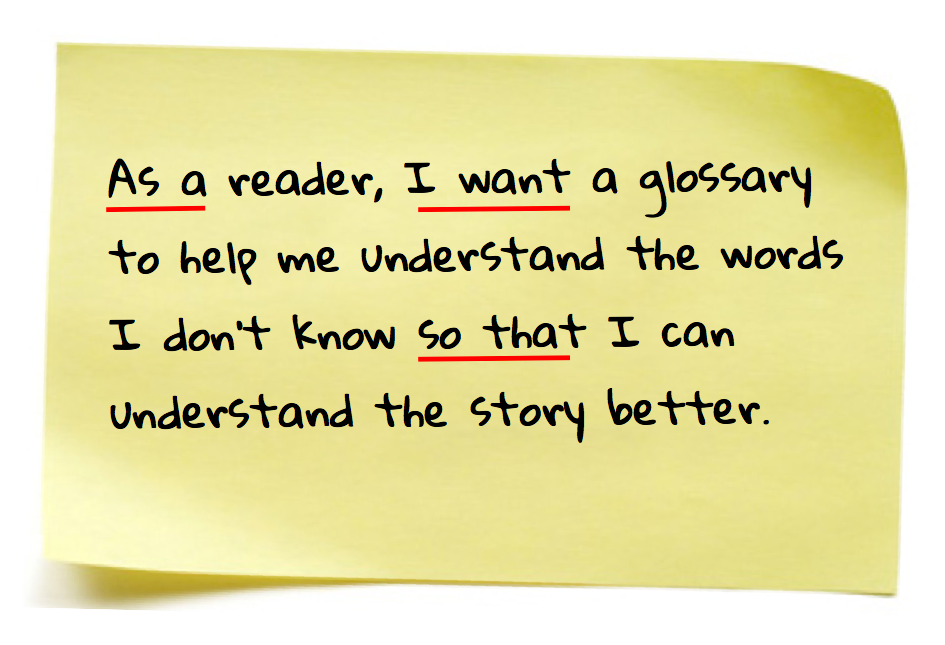
\includegraphics[width=0.7\linewidth]{./img/user-story}
\caption[Un esempio di \textit{user story}]{Un esempio di \textit{user story}}
\label{fig:user-story}
\end{figure}

La creazione delle storie, tipicamente, avviene in collaborazione con il cliente. Durante questo processo l'\textit{owner} lo guida, attraverso domande specifiche, alla stesura e formalizzazione delle funzionalit� necessarie.

Ogni storia rappresenta una feature ben precisa sviluppabile in un periodo che va, tipicamente, da alcuni giorni a un paio di settimane.

L'operazione fisica di scrittura della user story, aiuta il cliente a concretizzare la sua idea di progetto, visualizzandone i dettagli del funzionamento. Questo � molto utile sia per gli sviluppatori, sia per il cliente stesso. Infatti, spesso, i requisiti richiesti non sono dettagliati e specifici a sufficienza. Come ulteriore vantaggio si ha la costruzione di un linguaggio comune, condiviso, tra cliente e sviluppatori che rende agevole la realizzazione dell'intero progetto e dei futuri feedback.

Nel caso in cui le esigenze di progetto cambino, � molto facile, in questo processo, sia sostituire le user story, sia rendersi conto di quale impatto comporti il cambiamento, sull'intero sistema. 

Come sar� descritto nella sezione successiva, l'utilizzo delle user story si lega a quello del TDD, poich� i \textit{test} diverranno la dimostrazione oggettiva dell'effettiva implementazione e garanzia di correttezza di ogni storia.\\

\begin{figure}[h]
\centering
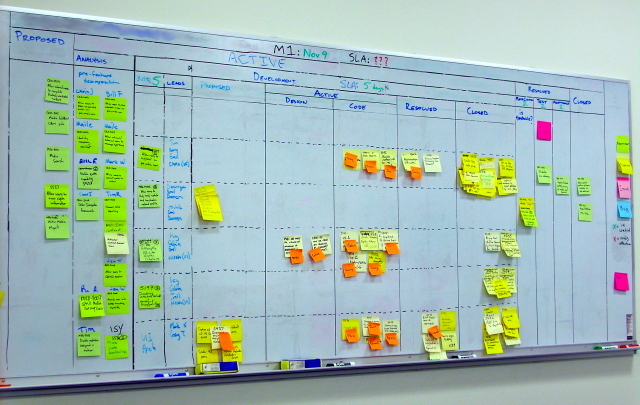
\includegraphics[width=1\linewidth]{./img/board}
\caption[Una lavagna con user story]{Una lavagna con user story}
\label{fig:board}
\end{figure}

	\clearpage
	\section{Il Test Driven Development}\label{Il_test_driven_development}
	Durante lo sviluppo del progetto ci siamo affidati al test driven development per avere la garanzia del comportamento atteso.

Il test driven development (TDD) � una tecnica di programmazione che prevede la scrittura di un test, ovvero di una porzione di codice che si occupa di verificare una funzionalit�, prima della stesura della funzionalit� stessa.

>per scrivere i test si utilizzano appositi \textit{framework} specifici per ogni linguaggio.

>I test posso essere soddifatti e sono definiti green o falliti e sono definiti red, questa nomenclatura deriva dalle usuali convenzioni degli ambienti di test che utilizzano questi colori per rappresentare il successo o meno di un test.

L'ideazione e la diffusione di questa tecnica di programmazione � stata curata da Kent Beck, che nel suo libro \textit{Test Driven Development: By Example} \cite{Beck:2002:TDD:579193} spiega come applicare il TDD a svariati contesti  legati allo sviluppo e dettaglia questa tecnica nelle sue tre fasi fondamentali definite abitualmente con il termine \textit{red-green-refactor}. Vediamo nel dettaglio cosa si intende con questo concetto.

\begin{description}
\item[Prima fase: red] Ogni nuova feature da implementare inizia con la stesura di un nuovo test, questo aiuta il programmatore a definire a priori le specifiche funzionali della porzione di sistema che dovr� implementare. La funzionalit� descritta dal test pu� mappare direttamente una \textit{user story} o pu� essere una porzione di essa. Non avendo implementato la funzionalit� il test sar� rosso (fallito). (verifica del test stesso?)
\item[Seconda fase: green] Questa fase del processo � quella nella quale si esegue lo sviluppo vero e proprio della funzionalit�, in modo da far diventare il test verde (soddisfatto). L'obbiettivo � esclusivamente soddisfare i requisiti, quindi tipicamente lo sviluppatore cerca di arrivare alla soluzione nel modo pi� semplice possibile, non curandosi dei dettagli stilistici del codice.
\item[Terza fase: refactor] L'ultimo passo da eseguire � la rifattorizzazione del codice, cio� la riorganizzazione delle funzionalit� realizzate al passo precedente al fine di ottenere una architettura ben congegnata e una struttura chiara. Una delle tecniche principali per realizzare questo compito � chiamata \textit{Don't Repeat Yourself} (DRY) e consiste nel cercare di rimuovere quanto pi� possibile codice duplicato mantenendo le stesse funzionalit�. L'utilizzo di questa tecnica favorisce il riuso e, tipicamente, veicola verso un buon design del software. In questa fase lo sviluppatore ha la massima libert� di sperimentazione, in quanto la correttezza del software rifattorizzato � garantita dai test scritti in precedenza. 
\end{description}

\begin{figure}[h]
\centering
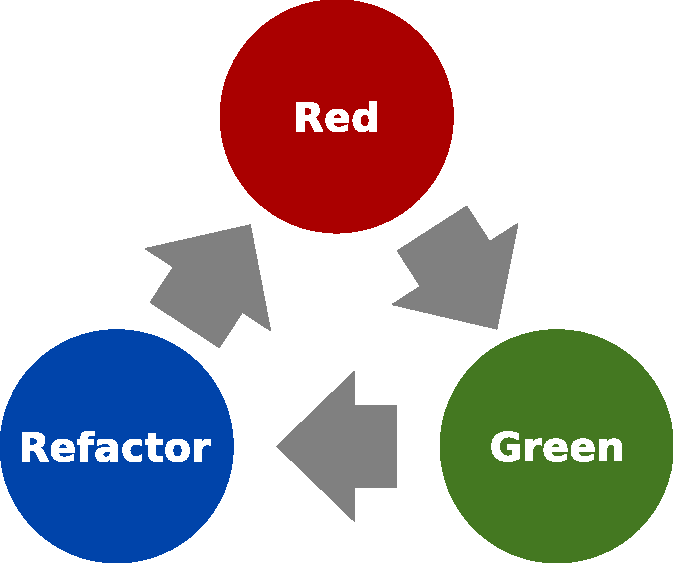
\includegraphics[width=0.7\linewidth]{./img/red-green-refactor}
\caption[Il flusso di lavoro del TDD]{Il flusso di lavoro del TDD}
\label{fig:red-green-refactor}
\end{figure}

Il processo � iterativo e ricomincia da capo

L'utilizzo del TDD fornisce allo sviluppatore svariati vantaggi, ad esempio:

- si riduce molto la necessit� di un debugger
- il programmatore acquisisce fiducia e non � pi� spaventato dal refactoring del codice, permette al programmatore di sperimentare soluzioni azzardate senza paura
- i test fungono da documentazione del codice e da traccia dello stato di avanzamento del progetto
- aiuta a modularizzare il codice e a realizzarlo in unit� indipendenti tra loro.
- favorisce il "concentrarsi sulle funzionalit�" e garantisce che ogni funzionalit� sia verificata con un test.




%TDD
%Il Test Driven Development, in sigla TDD (in italiano: Sviluppo guidato dalle verifiche) � un processo di sviluppo del software in cui lo sviluppo vero e proprio � preceduto (e guidato, driven) dalla stesura di test automatici.
%Sviluppato e diffuso da Kent Beck, fa parte delle 12 regole alla base dell'Extreme Programming (XP). Mentre XP � una metodologia agile, il TDD � una pratica agile.

%Il processo si articola sulla ripetizione di brevi cicli di sviluppo e collaudo (noti come "cicli TDD", TDD cycles) suddivisi in tre fasi successive, sintetizzate dal motto "Red-Green-Refactor".
%nella prima ("Red"), il programmatore scrive un test automatico (che necessariamente fallisce) per la funzionalit� da sviluppare.
%nella seconda ("Green"), il programmatore scrive la quantit� minima di codice necessaria per ottenere il superamento del test.
%nella terza, il programmatore ristruttura il codice (ovvero ne fa il refactoring).
%I colori "rosso" e "verde" si riferiscono alla rappresentazione grafica di fallimento e successo di un test automatico pi� diffusa negli IDE.
%Vantaggi
%Tali test permettono di individuare con precisione le specifiche del codice, e quindi il suo comportamento in base alle situazioni a cui sar� sottoposto. Ci� facilita la produzione di un codice funzionante in qualunque circostanza, pi� pulito e pi� affidabile.
%Scrivendo i test prima del codice, si utilizza il programma prima ancora che venga realizzato. Ci si assicura, inoltre, che il codice prodotto � testabile singolarmente. � dunque obbligatorio avere una visione precisa del modo in cui verr� utilizzato il programma prima ancora d'essere implementato. Cos� facendo si evitano errori concettuali durante la realizzazione dell'implementazione, senza che si siano definiti gli obiettivi. Inoltre, i test consentono agli sviluppatori di avere maggior confidenza durante il refactoring del codice, in quanto gi� sanno che i test funzioneranno quando richiesto; pertanto, possono permettersi di effettuare cambiamenti radicali di design, stando certi che alla fine otterranno un programma che si comporter� sempre alla stessa maniera (essendo i test sempre verificati).
%L'uso del Test Driven Development permette non solo di costruire il programma assieme ad una serie di test di regressione automatizzabili, ma anche di stimare in maniera pi� precisa lo stato d'avanzamento dello sviluppo di un progetto.

%------------------------------------------------------------------------------

%Test-driven development (TDD) is a software development process that relies on the repetition of a very short development cycle: first the developer writes an (initially failing) automated test case that defines a desired improvement or new function, then produces the minimum amount of code to pass that test, and finally refactors the new code to acceptable standards. Kent Beck, who is credited with having developed or 'rediscovered' the technique, stated in 2003 that TDD encourages simple designs and inspires confidence.[1]
%Test-driven development is related to the test-first programming concepts of extreme programming, begun in 1999,[2] but more recently has created more general interest in its own right.[3]
%Programmers also apply the concept to improving and debugging legacy code developed with older techniques.[4]

%The following sequence is based on the book Test-Driven Development by %Example.[1]
%Add a test[edit]
%In test-driven development, each new feature begins with writing a test. This test must inevitably fail because it is written before the feature has been implemented. (If it does not fail, then either the proposed "new" feature already exists or the test is defective.) To write a test, the developer must clearly understand the feature's specification and requirements. The developer can accomplish this through use cases and user stories to cover the requirements and exception conditions, and can write the test in whatever testing framework is appropriate to the software environment. This could also be a modification of an existing test. This is a differentiating feature of test-driven development versus writing unit tests after the code is written: it makes the developer focus on the requirements before writing the code, a subtle but important difference.
%Run all tests and see if the new one fails[edit]
%This validates that the test harness is working correctly and that the new test does not mistakenly pass without requiring any new code. This step also tests the test itself, in the negative: it rules out the possibility that the new test always passes, and therefore is worthless. The new test should also fail for the expected reason. This increases confidence (though does not guarantee) that it is testing the right thing, and passes only in intended cases.
%Write some code[edit]
%The next step is to write some code that causes the test to pass. The new code written at this stage is not perfect, and may, for example, pass the test in an inelegant way. That is acceptable because later steps improve and hone it.
%At this point, the only purpose of the written code is to pass the test; no further (and therefore untested) functionality should be predicted and 'allowed for' at any stage.
%Run tests[edit]
%If all test cases now pass, the programmer can be confident that the code meets all the tested requirements. This is a good point from which to begin the final step of the cycle.
%Refactor code[edit]
%Now the code should be cleaned up as necessary. Move code from where it was convenient for passing the test to where it logically belongs. Remove any duplication you can find. Make sure that variable and method names represent their current use. Clarify any constructs that might be misinterpreted. Use Kent Beck's four rules of simple design[5][6] to guide you, as well as anything else you know about writing clean code. By re-running the test cases, the developer can be confident that code refactoring is not damaging any existing functionality.
%The concept of removing duplication is an important aspect of any software design. In this case, however, it also applies to removing any duplication between the test code and the production code?for example magic numbers or strings repeated in both to make the test pass in step 3.
%Repeat[edit]
%Starting with another new test, the cycle is then repeated to push forward the functionality. The size of the steps should always be small, with as few as 1 to 10 edits between each test run. If new code does not rapidly satisfy a new test, or other tests fail unexpectedly, the programmer should undo or revert in preference to excessive debugging. Continuous integration helps by providing revertible checkpoints. When using external libraries it is important not to make increments that are so small as to be effectively merely testing the library itself,[3] unless there is some reason to believe that the library is buggy or is not sufficiently feature-complete to serve all the needs of the main program being written.

%Benefits[edit]

%A 2005 study found that using TDD meant writing more tests and, in turn, programmers who wrote more tests tended to be more productive.[11] Hypotheses relating to code quality and a more direct correlation between TDD and productivity were inconclusive.[12]
%Programmers using pure TDD on new ("greenfield") projects reported they only rarely felt the need to invoke a debugger. Used in conjunction with a version control system, when tests fail unexpectedly, reverting the code to the last version that passed all tests may often be more productive than debugging.[13]
%Test-driven development offers more than just simple validation of correctness, but can also drive the design of a program.[citation needed] By focusing on the test cases first, one must imagine how the functionality is used by clients (in the first case, the test cases). So, the programmer is concerned with the interface before the implementation. This benefit is complementary to Design by Contract as it approaches code through test cases rather than through mathematical assertions or preconceptions.
%Test-driven development offers the ability to take small steps when required. It allows a programmer to focus on the task at hand as the first goal is to make the test pass. Exceptional cases and error handling are not considered initially, and tests to create these extraneous circumstances are implemented separately. Test-driven development ensures in this way that all written code is covered by at least one test. This gives the programming team, and subsequent users, a greater level of confidence in the code.
%While it is true that more code is required with TDD than without TDD because of the unit test code, the total code implementation time could be shorter based on a model by M�ller and Padberg.[14] Large numbers of tests help to limit the number of defects in the code. The early and frequent nature of the testing helps to catch defects early in the development cycle, preventing them from becoming endemic and expensive problems. Eliminating defects early in the process usually avoids lengthy and tedious debugging later in the project.
%TDD can lead to more modularized, flexible, and extensible code. This effect often comes about because the methodology requires that the developers think of the software in terms of small units that can be written and tested independently and integrated together later. This leads to smaller, more focused classes, looser coupling, and cleaner interfaces. The use of the mock object design pattern also contributes to the overall modularization of the code because this pattern requires that the code be written so that modules can be switched easily between mock versions for unit testing and "real" versions for deployment.
%Because no more code is written than necessary to pass a failing test case, automated tests tend to cover every code path. For example, for a TDD developer to add an else branch to an existing if statement, the developer would first have to write a failing test case that motivates the branch. As a result, the automated tests resulting from TDD tend to be very thorough: they detect any unexpected changes in the code's behaviour. This detects problems that can arise where a change later in the development cycle unexpectedly alters other functionality.
%Madeyski [15] provided an empirical evidence (via a series of laboratory experiments with over 200 developers) regarding the superiority of the TDD practice over the classic Test-Last approach, with respect to the lower coupling between objects (CBO). The mean effect size represents a medium (but close to large) effect on the basis of meta-analysis of the performed experiments which is a substantial finding. It suggests a better modularization (i.e. a more modular design), easier reuse and testing of the developed software products due to the TDD programming practice.[15]
%Madeyski also measured the effect of the TDD practice on unit tests using branch coverage (BC) and mutation score indicator (MSI)[16] [17] ,[18] which are indicators of the thoroughness and the fault detection effectiveness of unit tests, respectively. The effect size of TDD on branch coverage was medium in size and therefore is considered substantive effect.[15]



%-----------------------------------------------------------------------------

%BDD
%Nell'ambito dell'ingegneria del software, il behavior-driven development (abbreviato in BDD e traducibile in Sviluppo guidato dal comportamento) � una metodologia di sviluppo del software basata sul test-driven development (TDD)[1][2] Il BDD combina le tecniche generali e i principi del TDD con idee prese dal domain-driven design e dal desing e all'analisi orientato agli oggetti per fornire agli sviluppatore software e ai Business analysts degli strumenti e un processo condivisi per collaborare nello sviluppo software.[1][3]
%Per quanto BDD sia principalmente un'idea di come lo sviluppo del software dovrebbe essere gestito sia da interessi di business e analisi tecniche, la pratica della BDD assume l'utilizzo di strumenti software specializzati per supportare il processo di sviluppo.[2] Sebbene questi strumenti siano spesso sviluppati in particolare per essere utilizzati in progetti BDD, possono essere visti anche come delle forme specializzate degli strumenti che supportano la TDD. Gli strumenti servono per aggiungere automazione all'ubiquitous language che � il tema centrale della BDD.

%------------------------------------------------------------------------------

%In software engineering, behavior-driven development (abbreviated BDD) is a software development process based on test-driven development (TDD).[1][2] Behavior-driven development combines the general techniques and principles of TDD with ideas from domain-driven design and object-oriented analysis and design to provide software developers and business analysts with shared tools and a shared process to collaborate on software development,[1][3] with the aim of delivering "software that matters".[4]
%Although BDD is principally an idea about how software development should be managed by both business interests and technical insight, the practice of BDD does assume the use of specialized software tools to support the development process.[2] Although these tools are often developed specifically for use in BDD projects, they can be seen as specialized forms of the tooling that supports test-driven development. The tools serve to add automation to the ubiquitous language that is a central theme of BDD.
	\clearpage

\chapter{Tecnologie Utilizzate}\label{Tecnologie_utilizzate}
In questo capitolo verranno approfonditi i dettagli delle tecnologie utilizzate per realizzare Mole.io. Saranno illustrate, per ognuna di esse, le motivazioni che ci hanno spinto alla scelta di particolari soluzioni software e le problematiche incontrate durante il loro utilizzo.

Il primo aspetto interessante dello sviluppo di Mole.io � il linguaggio di programmazione utilizzato per realizzarlo. L'intera applicazione infatti � stata sviluppata utilizzando il linguaggio \textit{JavaScript} (JS).

JavaScript � un linguaggio di \textit{scripting} dinamico, comunemente utilizzato, all'interno del browser, come supporto alla realizzazione di pagine web. Le sue applicazioni sono svariate: dall'animazione di porzioni di interfaccia grafica, alla comunicazione asincrona con il server, alla realizzazione di interi giochi all'interno del browser.

JS � un linguaggio \textit{prototype-based}, utilizza tipizzazione dinamica delle variabili, e presenta funzioni \textit{first-class}, � possibile infatti passarle come parametri, assegnarle ad una variabile e restituire valori da una funzione.

E' un linguaggio molto contaminato, la sua sintassi infatti si ispira a quella del C e di Java, ma utilizza alcuni principi di design provenienti dai linguaggi Lisp e Scheme \ref{osmani2012learning}. Questo fa si che JavaScript possa supportare differenti stili di programmazione, � infatti adatto ad essere utilizzato sia come linguaggio imperativo, sia Object Oriented, sia funzionale \ref{fogus2013functional}. 

Negli ultimi anni il mondo IT ha assistito ad una serie di utilizzi alternativi di JavaScript, ci sono state infatti applicazioni di questo linguaggio negli ambiti \textit{desktop}, \textit{mobile} ed \textit{embedded}.

L'aspetto pi� interessante, ai fini della realizzazione del progetto di tesi, � l'utilizzo di JS per la realizzazione di applicazioni \textit{server-side}. Questo approccio permette di ottenere un intero \textit{stack} applicativo uniforme che facilita la manutenzione dell'applicazione stessa. 

Uniformare il linguaggio utilizzato permette di facilitare lo sviluppo e la fruibilit� del progetto da parte degli sviluppatori. Per poter lavorare al software � infatti richiesta solo la conoscenza di JavaScript e non di altri linguaggi. Questo � un ottimo requisito quando se si immagina di avere a che fare con un team di sviluppo in espansione.

%JavaScript (JS) is a dynamic computer programming language.[5] It is most commonly used as part of web browsers, whose implementations allow client-side scripts to interact with the user, control the browser, communicate asynchronously, and alter the document content that is displayed.[5] It has also become common in server-side programming, game development and the creation of desktop applications.
%JavaScript is a prototype-based scripting language with dynamic typing and has first-class functions. Its syntax was influenced by C. JavaScript copies many names and naming conventions from Java, but the two languages are otherwise unrelated and have very different semantics. The key design principles within JavaScript are taken from the Self and Scheme programming languages.[6] It is a multi-paradigm language, supporting object-oriented,[7] imperative, and functional[1][8] programming styles.
%The application of JavaScript to use outside of web pages?for example, in PDF documents, site-specific browsers, and desktop widgets?is also significant. Newer and faster JavaScript VMs and platforms built upon them (notably Node.js) have also increased the popularity of JavaScript for server-side web applications. On the client side, JavaScript was traditionally implemented as an interpreted language but just-in-time compilation is now performed by recent (post-2012) browsers.
%JavaScript was formalized in the ECMAScript language standard and is primarily used as part of a web browser (client-side JavaScript). This enables programmatic access to computational objects within a host environment.

% JSON -> Douglas Crockford \ref{crockford2008javascript}

La piattaforma Node.js permette di utilizzare JavaScript per sviluppare la parte \textit{backend} delle applicazioni. 

Per il salvataggio dei dati, la scelta � ricaduta su MongoDB, un database documentale \textit{schema-less}, che permette di salvare dati direttamente in formato \textit{JavaScript Object Notation} (JSON). La possibilit� salvare nel database strutture dati gestite nativamente da JavaScript facilita notevolmente il lavoro di gestione delle informazioni. 

Il deploy in produzione di Mole.io verr� eseguito in un ambiente di tipo PaaS. Sistemi di questo tipo sono caratterizzati dalla possibilit� di fornire all'utente \textit{container} virtuali o macchine virtuali nelle quali eseguire le applicazioni. 

Quando si realizza il design di applicazioni per sistemi PaaS, quindi, � importante riuscire ad identificare i sotto-componenti software e gli specifici ruoli e compiti di ciascuno di essi. I sotto-sistemi devono quindi essere realizzati in modo da cooperare tra loro. Il \textit{disaccoppiamento} dei diversi servizi permette di scalare il sistema in modo da adattarne la configurazione alle specifiche esigenze in ogni istante.   

Una volta determinate le diverse componenti del sistema � necessario metterle in comunicazione tra di loro in modo da permettere la cooperazione e lo scambio di informazioni. A questo scopo si � deciso di introdurre nell'architettura applicativa RabbitMQ, una piattaforma per la gestione di code di messaggi, che permette lo scambio di dati tra le diverse componenti del sistema.

Il panorama attuale delle tecnologie per la realizzazione di applicazioni web \textit{client-side} � vastissimo. Per la costruzione di Mole.io la scelta � ricaduta su AngularJS, un popolare \textit{framework} sviluppato da Google appositamente per la creazione di \textit{single-page application}. Questo strumento � stato scelto principalmente a causa della sua naturale attitudine a lavorare con interfacce di \textit{backend} di tipo REST.     

Per lo sviluppo dell'interfaccia grafica si � scelto di utilizzare Bootstrap, un framework css che facilita la realizzazione e la stilizzazione di pagine web fornendo un \textit{set} di classi css preconfigurate. Questo ha permesso di realizzare velocemente un prototipo dell'applicazione con una interfaccia grafica decorosa. Le varie librerie JavaScript necessarie per il funzionamento dell'interfaccia sono state organizzate utilizzando \textit{Bower}, un tool per la gestione delle dipendenze.

Come strumento per il deploy dell'applicazione, si � scelto di utilizzare \textit{dokku}. Dokku � un software che permette di eseguire la posa in produzione dell'intera applicazione con un singolo comando lanciato direttamente dalla directory del repository di lavoro.

Nelle sezioni seguenti saranno mostrate nel dettaglio alcune delle tecnologie utilizzate per realizzare e mettere in produzione Mole.io.
	\clearpage
	\section{Node.js}\label{Nodejs}
	La \textit{homepage} del sito ufficiale di Node.js \cite{website:Node.js} fornisce una sintetica ma precisa descrizione di questa tecnologia, un buon punto di partenza per illustrarne le peculiarit�.\\

\begin{figure}[h]
\centering

\includegraphics[width=0.7\linewidth]{./img/nodejs-light}
\caption[Il logo ufficiale di Node.js]{Il logo ufficiale di Node.js}
\label{fig:nodejs-light}
\end{figure}

La descrizione di Node.js riportata sul sito recita:

\begin{quote}
\textit{Node.js is a platform built on Chrome's JavaScript runtime for easily building fast, scalable network applications. Node.js uses an event-driven, non-blocking I/O model that makes it lightweight and efficient, perfect for data-intensive real-time applications that run across distributed devices.}
\end{quote}

E' immediato comprendere che Node.js � una \textit{piattaforma}. L'utilizzo di questo termine mette l'accento su un aspetto fondamentale di questa tecnologia: fornire un ambiente nel quale le applicazioni sviluppate possano funzionare con il supporto di librerie di sistema fornite da Node.js stesso.

La piattaforma Node.js utilizza JavaScript come linguaggio di sviluppo. Per farlo si avvale di una versione appositamente riadattata del potente interprete \textit{V8} presente all'interno del browser \textit{Chrome} di \textit{Google}. L'utilizzo di un linguaggio altamente diffuso e di una base solida come quella fornita dal popolare \textit{browser} permettono di costruire applicazioni affidabili in modo semplice e veloce.

L'ultimo importante concetto, che si apprende dalla prima frase della descrizione, � che Node.js � principalmente orientato allo sviluppo di applicazioni che lavorano con la rete. Per sua natura, la piattaforma ci aiuta a fare in modo che esse siano facilmente scalabili.

La seconda parte della descrizione spiega sinteticamente alcune caratteristiche peculiari di Node.js e ne definisce meglio il contesto applicativo. 

L'intera piattaforma � centrata sul concetto di \textit{evento}. Si dice  evento un messaggio che viene scatenato in un determinato istante dell'elaborazione e che successivamente � catturato e gestito dalle componenti del sistema che sono preposte alla gestione di quell'evento specifico.

Il sistema ad eventi viene utilizzato da Node.js congiuntamente ad una gestione non bloccante delle operazioni di \textit{Input/Output}. Questo significa che una operazione potenzialmente lunga, come ad esempio la comunicazione con il \textit{filesystem} o con i dispositivi di \textit{rete}, non blocca il flusso di esecuzione del programma principale.

Dopo aver richiesto ad altri attori del sistema il dato di cui necessita, il programma continua il suo normale flusso di esecuzione e verr� informato, utilizzando un evento, quando il dato richiesto sar� disponibile. Questa gestione non bloccante delle operazioni di \textit{I/O} � chiamata \textit{I/O asincrono}.

La gestione delle operazioni in modo non strettamente legato alla logica applicativa, permette a Node.js di essere molto efficiente se utilizzato per la realizzazione di applicazioni che manipolano grandi quantit� di dati, ma devono rimanere \textit{reattive} nei confronti di nuove richieste di elaborazione.

\subsection{Le operazioni asincrone}

Interessante, a fronte dell'introduzione del concetto di I/O asincrono, � vedere come Node.js riesca a gestirlo utilizzando una quantit� limitata di risorse di sistema.

I componenti \textit{hardware} di un sistema elaborano dati con velocit� differenti. La rapidit� di ogni componente � fortemente legata al modo nel quale questo � stato realizzato. La tabella seguente riporta un elenco di componenti e le relative velocit� indicative riferite ad un singolo ciclo di \textit{CPU}. 

\begin{center}
\begin{tabular}{l|r}
\textbf{Componente} & \textbf{Numero di cicli} \\ 
\hline 
CPU & 1 \\ 
Cache di livello 1 & 3 \\ 
Cache di livello 2 & 14 \\ 
RAM & 250 \\ 
Hard Disk & 41.000.000 \\ 
Dispositivo di rete & 240.000.000 \\ 
\end{tabular} 
\end{center}

Guardando la tabella si nota immediatamente come i dispositivi di \textit{I/O} siano ordini di grandezza pi� lenti rispetto ai dispositivi di elaborazione delle informazioni. Se il flusso del programma dovesse aspettare, in modo sincrono, ogni singola operazione di lettura o scrittura su disco, ad esempio, esso perderebbe la possibilit� di eseguire circa quaranta milioni di operazioni di calcolo, con un conseguente degrado delle performances del software.

Una tecnica comune per affrontare il problema dell'\textit{I/O} � l'utilizzo di \textit{threads}. Un thread � spesso definito con il termine "sotto-processo leggero", in effetti esso condivide codice e risorse di sistema con altri threads appartenenti allo stesso processo padre.

L'utilizzo dei thread permette ad un processo di parallelizzare l'esecuzione di una parte del suo flusso di lavoro. Al tempo stesso sono necessarie risorse di sistema sia per creare il thread sia per distruggerlo. Node.js ovvia a questo problema utilizzando un \textit{thread pool}, cio� un insieme di thread che fungono da \textit{worker} per il processo. Quando � necessario eseguire un particolare \textit{task}, esso viene sottoposto al thread pool, di conseguenza viene assegnato ad un worker. Esso lo esegue e al termine del lavoro comunica l'esito dell'elaborazione al chiamante tramite una funzione detta \textit{callback}.

L'utilizzo di un thread pool comporta un incremento di prestazioni da parte delle applicazioni che lo sfruttano: i thread pool ottimizzano l'utilizzo della memoria e del processore, diminuendo l'overhead di gestione dei thread.

Per comprendere come Node.js sia in grado di realizzare tale funzionalit�, � necessario spiegare nel dettaglio il modello di gestione delle richieste implementato da questo framework. 

Innanzitutto � necessario chiarire che Node.js, a differenza di altri sistemi per lo sviluppo \textit{server-side} non necessita di una applicazione che funga da \textit{web server}, come accade ad esempio nel caso di Apache per PHP. Quando si sviluppa in Node.js infatti l'applicazione realizzata \textit{�} il server. Il framework mette a disposizione funzionalit� apposite per la creazione di un server interno ad ogni applicazione. Questo approccio favorisce la strutturazione a \textit{servizi} dell'applicazione, che pu� essere suddivisa in processi Node.js separati e quindi in veri e propri server in comunicazione fra loro.

Di seguito � riportato un server web minimale realizzato in Node.js.

\begin{verbatim}
var http = require('http');

http.createServer(function (req, res) {
  res.end('Hello World');
}).listen(3000, '127.0.0.1');

console.log('Server running at http://127.0.0.1:3000/');
\end{verbatim}

La prima operazione eseguita dal programma � l'importazione del modulo \verb|http|, che fornisce le funzionalit� di rete. Successivamente viene chiamata la funzione \verb|createServer()| che si occupa di generare il server web. Utilizzando la funzione \verb|listen()|, successivamente, il server viene attivato e messo in ascolto all'indirizzo \verb|http://127.0.0.1:3000/|. Il comando \verb|console.log()| stampa in console l'informazione che il server � avviato. Ad ogni richiesta ricevuta dal server, viene eseguita la funziona passata come parametro alla \verb|createServer()|, la quale risponde alla richiesta inviando al client la stringa \verb|Hello World|.

Come si vede da questo esempio, con Node.js, la logica applicativa e il \textit{web-server} risiedono all'interno dello stesso software.

Node.js utilizza internamente un modello chiamato \textit{Event Loop} per la gestione delle richieste in arrivo. All'avvio dell'applicazione, vengono attivati un thread principale e un insieme finito (il default � quattro) di thread secondari definiti \textit{thread-pool}. Nell'istante in cui arriva una nuova richiesta da parte di un client, il thread principale la prende in carico ed inserisce i dati della richiesta e la funzione \textit{callback} per gestirla in una coda. A fronte di questa operazione, viene attivato il primo thread libero nel thread-pool, detto \textit{worker}, il quale esegue la callback e raccoglie il risultato. Una volta generato il messaggio di risposta da inviare al client, il worker lo restituisce al thread principale, il quale provvede ad inviarlo al client.

Questo approccio presenta un grande vantaggio rispetto ad altri sistemi non \textit{event-based}: il thread principale � quasi sempre in stato \textit{idle}. Esso si occupa infatti esclusivamente di smistare richieste e raccogliere risposte, quindi rimane sempre reattivo. Il risultato di questo approccio � un sistema responsivo, che riesce a gestire un grande numero di richieste sfruttando una bassissima quantit� di risorse di sistema.

In figura \ref{fig:node-model} � illustrato schematicamente l'event-loop per la gestione delle richieste di Node.js.

\begin{figure}[h]
\centering
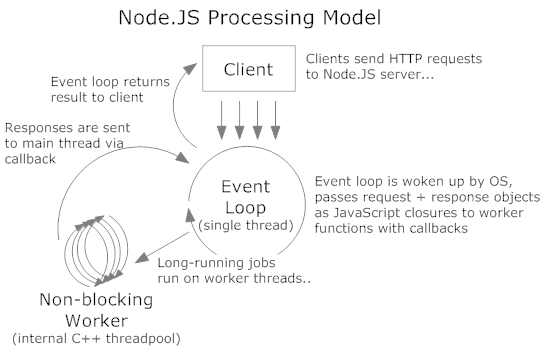
\includegraphics[width=0.7\linewidth]{./img/node-model}
\caption[L'\textit{event loop} di Node.js]{L'\textit{event loop} di Node.js}
\label{fig:node-model}
\end{figure}

\subsection{Le callback}

Una delle principali difficolt� che si presenta ad uno sviluppatore che si appresta ad utilizzare Node.js per la prima volta, � la gestione delle callback. Di seguito � riportato un frammento di codice Node.js che esegue il salvataggio di un utente su Database.

\begin{verbatim}
function save(user) {
  console.log('saving user into db');
  db.insert(user, function(err, user) {
    console.log('user successfully saved!');
  });
  console.log('all we need is just a little patience...');
}
\end{verbatim}

la funzione \verb|db.insert()| � asincrona, ed accetta due parametri: il dato da salvare e la callback da eseguire una volta effettuato l'inserimento nel Database. L'esecuzione di questo codice produce un output in console simile a quello mostrato qui sotto.

\begin{verbatim}
saving user into db
all we need is just a little patience...
user successfully saved!
\end{verbatim}

Se la funzione \verb|db.insert()| non fosse asincrona otterremmo un output come quello che segue.

\begin{verbatim}
saving user into db
user successfully saved!
all we need is just a little patience...
\end{verbatim}

Questo piccolo esempio, lascia intuire un potenziale problema nella gestione delle callback: se, ad esempio, dovessimo assegnare alcuni privilegi di \textit{default} a tutti i nuovi utenti inseriti nel sistema, potremmo scrivere il seguente codice.

\begin{verbatim}
function save(user) {
  console.log('saving user into db');
  db.insert(user, function(err, user) {
  	db.insert(grants, user, function(err, grants) {
      console.log('user successfully saved!');
    });
  });
  console.log('all we need is just a little patience...');
}
\end{verbatim}

Ora il problema � evidente: se i dati ottenuti in modo asincrono sono necessari per eseguire altre procedure, essi vanno gestiti internamente alla callback stessa. Se utilizzate in modo improprio, le callback, portano al cosiddetto \textit{callback-hell}, ovvero un codice nel quale il lettore non riesce pi� a seguire il flusso logico dell'applicazione.

Fortunatamente JavaScript ci fornisce una soluzione semplice al problema, ma che richiede allo sviluppatore disciplina nello scrivere il codice sorgente. L'esempio precedente, infatti potrebbe essere riscritto come segue.

\begin{verbatim}
function onGrantsSaved(err, grants) {
  console.log('user successfully saved!');
}

function onUserSaved(err, user) {
  db.insert(grants, user, onGrantsSaved);
}

function save(user) {
  console.log('saving user into db');
  db.insert(user, onUserSaved);
  console.log('all we need is just a little patience...');
}
\end{verbatim}

Il codice � ora molto pi� leggibile, semplicemente evitando la dichiarazione di funzioni anonime in linea. 

% js nel server
%Questo � un aspetto molto controverso e discusso, infatti se � abituati 
%a pensare tale linguaggio come un "giocattolo", troppo instabile 
%e imprevedibile per 


	\clearpage
		\subsection{Npm e Moduli}\label{Npm_e_moduli}
		L'organizzazione del codice � un aspetto fondamentale dello sviluppo. Il \textit{Single Responsibility Principle} (SRP) � uno dei principi di design del software pi� importanti. Applicato alla programmazione ad oggetti, esso sostiene che ogni oggetto deve essere responsabile di un singolo aspetto del comportamento del sistema. 

Node.js incarna questo principio nelle fondamenta della sua struttura, infatti permette di organizzare il codice in unit� indipendenti tra loro chiamate \textit{moduli}. Ogni modulo nella piattaforma pu� decidere quali dati gestire al suo interno e quali esporre all'esterno. Si creano in questo modo delle \textit{black box} che funzionano tanto meglio quanto il loro compito � specifico. 

Poco dopo la nascita di Node.js la comunit� di sviluppatori che lo utilizzava ha deciso di arricchire questa piattaforma con un \textit{tool} ormai insostituibile: \textit{Node Package Manager} (NPM).\\

\begin{figure}[h]
\centering

\includegraphics[width=0.7\linewidth]{./img/npm}
\caption[Il logo di NPM]{Il logo di NPM}
\label{fig:npm}
\end{figure}

NPM \cite{website:NPM} � un tool, utilizzabile da linea di comando, che si occupa della gestione dei moduli e delle loro dipendenze, per farlo utilizza un \textit{repository} in rete nel quale sono registrati tutti i moduli pubblici sviluppati dai vari \textit{contributor} della \textit{community} Node.js.

Abbiamo introdotto il concetto di \textit{dipendenza} tra moduli. Un modulo si dice dipendente da un altro quando necessita di quest'ultimo per eseguire il suo compito. NPM impone che ogni modulo sia descritto dal file \verb|Package.json| che ne riporta le informazioni principali ed elenca gli altri moduli dai quali dipende. Di seguito riportiamo un esempio di \verb|Package.json| per un modulo chiamato \verb|mole| che fa parte del sistema realizzato per questa tesi.

\begin{verbatim}
{
  "name": "mole",
  "version": "0.0.1",
  "author": "Federico Gandellini",
  "description": "whisper collector and denormalizer",
  "private": true,
  "scripts": {
    "start": "node mole.js"
  },
  "engines": {
    "node": ">=0.8.0",
    "npm": ">=1.2.0"
  },
  "dependencies": {
    "express": "3.3.4",
    "underscore": "~1.5.2",
    "mongo-make-url": "0.0.1",
    "mongoskin": "~0.6.0",
    "mongodb": "~1.3.19",
    "require-all": "0.0.8",
    "rabbit.js": "~0.3.1"
  },
  "devDependencies": {
    "grunt-contrib-jshint": "~0.6.4",
    "grunt": "~0.4.1",
    "grunt-mocha-cli": "~1.2.1",
    "grunt-contrib-watch": "~0.5.3",
    "mocha": "~1.13.0",
    "should": "~1.3.0",
    "supertest": "~0.8.0",
    "Faker": "~0.5.11"
  }
}
\end{verbatim}

Nella prima parte del file possiamo trovare i dati principali del modulo, come il suo nome, l'autore, la versione, e una descrizione. Seguono un paio di parametri che definiscono le regole di pubblicazione, il comando per lanciare questo modulo e le versioni richieste della piattaforma Node.js e di NPM.

Le due sezioni seguenti nel file elencano le dipendenze, la prima indica i moduli che devono essere presenti perch� esso possa essere messo \textit{in produzione}, le altre sono dipendenze che sono richieste esclusivamente durante lo sviluppo o il \textit{testing} del modulo stesso. Come si pu� notare, nel file, non sono presenti solo i nomi, ma anche le versioni richieste degli altri moduli.

Uno dei comandi di NPM pi� utilizzati � \verb|npm install|. Il comando indica a NPM di leggere il file \verb|Package.json| presente nella \textit{directory} corrente e scaricare dalla rete tutti i pacchetti richiesti alle rispettive versioni. In questo modo, l'utilizzatore del modulo � immediatamente operativo.

\subsubsection{Alcuni moduli utilizzati}

Per poter utilizzare le funzionalit� fornite da un modulo aggiuntivo, Node.js fornisce un comando che permette di importarlo dall'esterno. Questo comando � \verb|require()| e si utilizza passando come parametro il nome del modulo da caricare. 

\begin{verbatim}
var express = require('express');
\end{verbatim}

Una volta eseguito il comando, la variabile \verb|express| conterr� il modulo appena caricato e sar� possibile utilizzarne le funzionalit�.\\

Di seguito verranno presi in considerazione alcuni dei principali moduli utilizzati per realizzare l'applicazione oggetto della tesi.
\begin{description}
\item [express] \`{E} uno dei moduli pi� importanti: permette di creare facilmente un \textit{server web} in grado di rispondere a richieste provenienti dai \textit{client}. Utilizza un sistema di \textit{rotte} per legare l'azione da eseguire alla richiesta HTTP in arrivo. Express eredita da \textit{Connect} una funzionalit� chiave per il suo funzionamento, i \textit{middleware}. In Connect, un middleware � una funzione che filtra tutte le richieste in ingresso e le risposte in uscita e le restituisce rielaborate. I middleware sono costruiti in modo da essere accodati l'uno con l'altro, dando la possibilit� di realizzare filtri molto complessi. La configurazione delle rotte e dei middleware di express verr� illustrata nella sezione \ref{Architettura_del_sistema}.
\item [passport] Il compito di questo modulo � gestire l'autenticazione degli utenti. Passport fornisce un comodo middleware per express, con il quale � possibile verificare i dati di autenticazione dell'utente quando questo voglia accedere a specifiche rotte. Pi� avanti, nella sezione \ref{Autenticazione_degli_utenti}, sar� approfondito questo tema.
\item [mongoose e mongoskin] Sono i due principali \textit{driver} Node.js per MongoDB, il sistema per l'archiviazione dei dati che abbiamo utilizzato nell'applcazione. Nella sezione \ref{MongoDB} verr� illustrato nel dettaglio questo database documentale e si mostrer� come � possibile accedere alla sua interfaccia utilizzando Node.js.
\item [require-all] Permette di caricare tutti i moduli presenti in una directory. Questo modulo ci � stato molto utile per garantire e semplificare l'estensibilit� del sistema. Nella sezione \ref{CQRS_ed_estensibilita} si analizzer� nel dettaglio come � stata sfruttata questa semplice ma potente funzionalit�.
\item [mocha] Questo modulo non fornisce funzionalit� vere e proprie da spendere in produzione, bens� un insieme preziosissimo di \textit{tool} per poter testare la propria applicazione Node.js. Tale strumento � stato largamente utilizzato durante la realizzazione del sistema, applicando le tecniche illustrate nel capitolo \ref{Il_test_driven_development}, per rendere Mole.io, quanto pi� possibile, \textit{bug-free}.
\end{description} 
		\clearpage
	\section{RabbitMQ}\label{RabbitMQ}
	Quando si progetta una applicazione web che offre un servizio, bisogna sempre porre molta attenzione a non introdurre nel sistema i cosiddetti \textit{colli di bottiglia}, cio� componenti dell'architettura che non riescono a sopportare il carico delle richieste in arrivo dagli utenti.

Una tecnica piuttosto efficace per evitare i colli di bottiglia, consiste nel realizzare un \textit{disaccoppiamento} delle varie componenti presenti nel sistema. Una applicazione ben disaccoppiata � una applicazione nella quale ogni singolo componente svolge una funzione specifica e comunica con le altre parti del sistema secondo protocolli predefiniti. Disaccoppiare quindi non � sempre facile, perch� � necessario costruire infrastrutture che permettano alle varie parti, ormai slegate, di comunicare tra loro.

RabbitMQ \cite{website:RabbitMQ} � un software che permette di realizzare, configurare e monitorare complessi sistemi di code di messaggi. Il suo utilizzo permette di realizzare una infrastruttura nella quale le diverse parti di un sistema possano comunicare tra loro scambiandosi messaggi attraverso le code utilizzando un protocollo determinato dallo sviluppatore.\\

\begin{figure}[h]
\centering

\includegraphics[width=0.7\linewidth]{./img/rabbit_header_logo}
\caption[Il logo di RabbitMQ]{Il logo di RabbitMQ}
\label{fig:rabbit-logo}
\end{figure}

L'utilizzo di RabbitMQ fornisce un vantaggio evidente in termini di flessibilit�: � possibile agganciare o rimuovere parti da un sistema attivo senza comprometterne l'intero funzionamento.

La flessibilit� non � l'unico vantaggio, infatti RabbitMQ permette di ottenere architetture perfettamente gestibili su sistemi di tipo \textit{Platform as a Service} (PaaS), sui quali si pu� decidere di aumentare o diminuire dinamicamente le risorse fornite ad un sistema in produzione in accordo con il numero di richieste utente da soddisfare. 

RabbitMQ permette di costruire \textit{pattern} di comunicazione tra processi, i pi� utilizzati sono quelli riportati di seguito.

\subsubsection{Work Queues}

L'idea alla base di questo tipo di configurazione, chiamata anche \textit{Task Queues}, consiste nell'evitare picchi nel carico di lavoro e risorse del sistema, dovuti allo svolgimento di una operazione e all'attesa del suo completamento. Per ovviare a questo problema si configura un sistema nel quale esiste un produttore di dati e uno o pi� consumatori.\\

\begin{figure}[h]
\centering
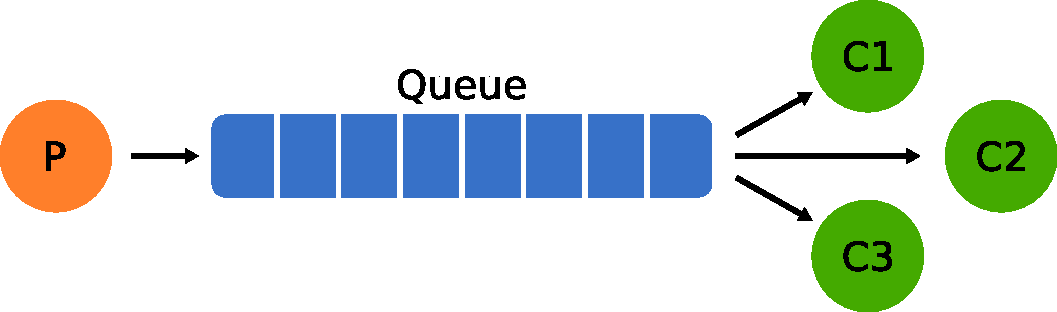
\includegraphics[width=0.7\linewidth]{./img/rabbit-workers}
\caption[Work Queues in RabbitMQ]{Work Queues in RabbitMQ}
\label{fig:rabbit-work-queues}
\end{figure}

In figura \ref{fig:rabbit-work-queues} vediamo una rappresentazione schematica di questo tipo di configurazione. All'arrivo di una richiesta di elaborazione, il produttore (P) invia un messaggio sulla coda. I consumatori (C1, C2 e C3) in attesa estraggono un messaggio dalla coda e lo elaborano.

Nella sua configurazione base, la coda esegue un \textit{load-balancing} dei messaggi, questo significa che fornisce esattamente lo stesso quantitativo di messaggi, e quindi di carico di lavoro, ad ogni consumatore.

RabbitMQ permette di variare il numero di consumatori in ascolto sulla coda dinamicamente, a \textit{runtime}. Non appena un nuovo consumatore si registra per la ricezione dei messaggi, il carico di lavoro viene automaticamente ricalcolato in modo da essere costante per tutti i nodi.

Il load-balancing automatico e la possibilit� di sottoscrivere consumatori a runtime diventano funzionalit� molto importanti in presenza di sistemi attivi su PaaS. All'aumentare delle richieste, infatti, il sistema potrebbe in automatico attivare nuovi consumatori e sottoscriverli, ottenendo in questo modo un sistema altamente scalabile. 

\subsubsection{Publish/Subscribe}

Questa configurazione si ispira al concetto di \textit{abbonamento}, l'idea di base infatti � poter inviare il medesimo messaggio a pi� destinatari.\\

\begin{figure}[h]
\centering
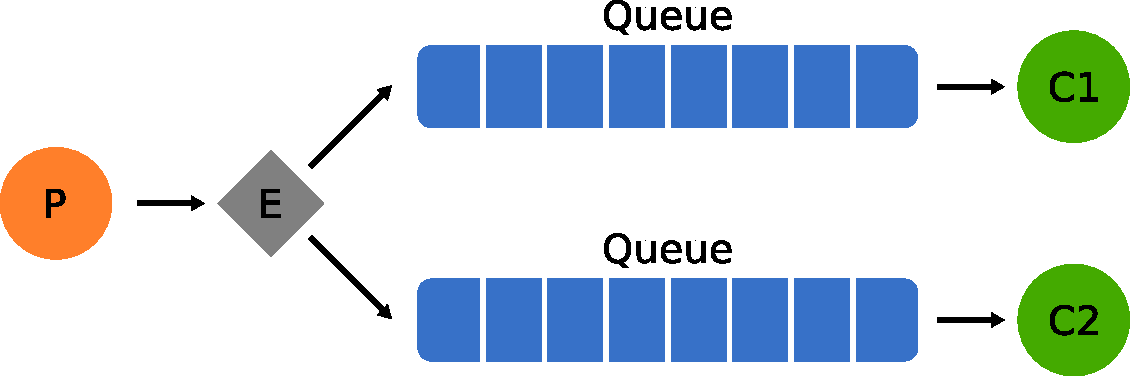
\includegraphics[width=0.7\linewidth]{./img/rabbit-pub-sub}
\caption[Publish/Subscribe in RabbitMQ]{Publish/Subscribe in RabbitMQ}
\label{fig:rabbit-publish-subscribe}
\end{figure}

La figura \ref{fig:rabbit-publish-subscribe} mostra una rappresentazione del sistema Publish/Subscribe. A differenza del modello \textit{Work Queues}, qui � stato aggiunto un nuovo attore: un \textit{exchange} (E) il cui compito � duplicare i messaggi e inviarli a tutte le code ad esso connesse.

In questo caso il produttore di messaggi (P) invia un messaggio ad un exchange (E), il quale lo duplica e lo invia a tutte le code ad esso connesse. I consumatori in ascolto (C1 e C2), riceveranno lo stesso messaggio.\\

Nella sezione \ref{Architettura_del_sistema} sar� illustrata nel dettaglio la configurazione di RabbitMQ utilizzata per realizzare Mole.io e quali tecniche si sono messe in atto per permettere al sistema di essere installato su una piattaforma di tipo PaaS. 
	\clearpage
	\section{MongoDB}\label{MongoDB}
	Il salvataggio dei dati � una operazione critica in moltissimi sistemi software. La scelta del tipo di database da utilizzare per salvare le informazioni � altrettanto delicata e va ponderata alla luce di svariati punti di vista. Per la realizzazione della applicazione oggetto di tesi, si � scelto di utilizzare MongoDB \cite{website:MongoDB}. Di seguito verranno illustrate le principali caratteristiche di questo database e le motivazioni che sottendono tale scelta.\\

\begin{figure}[h]
\centering

\includegraphics[width=0.7\linewidth]{./img/mongodb}
\caption[Il logo di MongoDB]{Il logo di MongoDB}
\label{fig:mongodb}
\end{figure}

I database relazionali (RDBMS), per loro natura, espongono il loro contenuto in un formato tabellare e utilizzano concetti come righe e colonne per fornire l'accesso ai dati o porzioni di essi. In questo tipo di database lo \textit{schema} dei dati, cio� la struttura delle informazioni � ben definita e va studiata in fase di \textit{design} della base di dati, essi si definiscono infatti database \textit{schema-full}. Negli RDBMS la modifica del formato di un dato a sistema avviato � una operazione delicata. Essa infatti deve tenere conto dei dati gi� presenti all'interno del sistema e deve aggiornarli coerentemente con la nuova struttura assunta dalla tabella che li contiene.

MongoDB � un database \textit{schema-less}, questo significa che la struttura di un dato non � definita a priori, ma soprattutto che essa pu� variare nel tempo senza richiedere aggiornamenti ai dati gi� presenti nella base dati. MongoDB utilizza infatti un modello documentale per la rappresentazione dei dati, essi sono salvati internamente come oggetti \textit{BSON} e forniti all'esterno sotto forma di oggetti \textit{JSON}.   

Per comprendere i concetti alla base di MongoDB � possibile realizzare alcune similitudini tra concetti proposti da questa base dati e concetti presenti negli RDBMS. La tabella seguente mostra alcune di queste similitudini.

\begin{center}
\begin{tabular}{l|l}
\textbf{RDBMS} & \textbf{MongoDB} \\ 
\hline 
table & collection \\ 
tuple & document \\ 
column & field \\
\end{tabular} 
\end{center}

Le \textit{collection} sono insiemi di \textit{document}, i quali, a loro volta, contengono vari \textit{field} che rappresentano le chiavi per l'accesso ai dati veri e propri: i \textit{value}.

Un documento BSON pu� contenere \textit{field} di vario tipo: interi, stringhe, \textit{array}, dati binari, oppure altri documenti (\textit{embedded document}). Come abbiamo anticipato, in MongoDB, lo schema dei documenti non � fisso, questo significa che nella stessa collection potremo trovare document con struttura differente.

Altre funzionalit� significative di MongoDB sono:
\begin{itemize}
\item la possibilit� di eseguire aggiornamenti atomici dei dati;
\item la ricerca \textit{full-text} all'interno di documenti e di \textit{embedded document};
\item la possibilit� di creare indici su dati;
\item la creazione di indici di tipo geospaziale;
\end{itemize}

Si � scelto questo tipo di database perch� fornisce la possibilit� di salvare dati aventi una struttura variabile. Nel capitolo \ref{mole} si vedr� come questa funzionalit� permette di creare un sistema estremamente flessibile.

I creatori di MongoDB hanno fatto in modo che il database da loro realizzato possedesse due caratteristiche fondamentali, che lo rendono il candidato ideale per l'installazione in ambienti PaaS: l'alta accessibilit� e la scalabilit�.

Nella sezione seguente si illustrer� come MongoDB implementa questi due concetti e come essi si possano utilizzare sia per fronteggiare l'aumento di richieste da parte degli utenti, sia per rendere il sistema resistente a problemi di malfunzionamento dei server sui quali MongoDB viene installato.

La sezione \ref{mole} fornir� inoltre elementi per comprendere come queste caratteristiche hanno reso MongoDB lo strumento pi� adatto ad essere integrato nell'applicazione oggetto di tesi. Nella configurazione finale, infatti, esso verr� installato proprio su un servizio di tipo PaaS.
	\clearpage
		\subsection{Fronteggiare le Richieste}\label{Fronteggiare_le_richieste}
		Come � stato anticipato, MongoDB � un database documentale che garantisce alte \textit{performance}, alta accessibilit� e permette facilmente di scalare la sua struttura per fronteggiare le richieste. Di seguito sar� descritto brevemente come MongoDB realizza ognuna di queste funzionalit�:

\begin{description}
\item[Database documentale] I documenti contenuti in MongoDB (oggetti) mappano molto bene gli oggetti e le strutture dati fornite dai principali linguaggi di programmazione, rendendo quasi inutile la necessit� di un software di traduzione tra strutture dati utilizzate nel software e la loro rappresentazione nel database. Tipicamente i software di \textit{Object-Relational Mapping} (ORM) sono necessari in presenza di database relazionali. Il vantaggio di avere gli \textit{embedded document}, inoltre, permette di ridurre il numero di operazioni di \textit{join} sui dati, rendendo superflua una delle caratteristiche fondamentali dei RDBMS. Con MongoDB diventa quindi molto semplice far \textit{evolvere} le proprie strutture dati, rendendo lo sviluppo dell'applicazione molto pi� flessibile.

\item[Alte \textit{performance}] La possibilit� di inserire documenti all'interno di altri documenti, garantisce scritture veloci e la definizione degli indici pu� includere chiavi presenti negli \textit{embedded documents}, in questo modo � possibile ottenere tempi di risposta del sistema molto contenuti.

\item[Alta accessibilit�] Questa propriet�, chiamata tecnicamente, \textit{High Availability} (HA), � realizzata con server replicati e organizzati in \textit{cluster}, detti \textit{replica-set}, nei quali � possibile identificare un \textit{master} e altri \textit{slave}. Il master riceve le richieste e le smista sugli slave nel cluster. In caso di problemi al server master, MongoDB esegue una elezione automatica del nuovo master tra gli slave rimanenti.

\item[Facile scalabilit�] Lo \textit{sharding} � la possibilit� di suddividere una collection su pi� server in modo automatico. Questa caratteristica rende MongoDB altamente indicato per essere installato su piattaforme di tipo PaaS, all'aumentare dei dati presenti nel database, infatti, � sufficiente aumentare il numero di server a disposizione per accogliere pi� informazioni. Dal punto di vista dell'applicazione che utilizza questi dati, questa operazione � trasparente. In questo modo il numero di server necessari aumenta linearmente all'aumentare della quantit� di dati salvata. \`{E} possibile aggiungere server in modo dinamico, senza arrestare il sistema, questa funzionalit� � particolarmente importante quando MongoDB � utilizzato per contenere dati di applicazioni web che non ammettono momenti di \textit{downtime}. 
%parlare di eventual consistency? \cite{Vogels:2008:EC:1466443.1466448}
%Eventually-consistent reads can be distributed over replicated servers.
\end{description}

Oltre alla flessibilit� offerta dal modello documentale, MongoDB include le funzionalit� comuni degli RDBMS, quali indici, aggregazioni, \textit{query}, ordinamenti, aggiornamenti di dati aggregati e \textit{upsert}, cio� aggiornamento di un dato se gi� esistente o creazione di un nuovo dato. 

Gli sviluppatori di MongoDB hanno cercato di realizzare un database che fosse semplice da installare e manutenere, infatti la filosofia alla base di MongoDB � "fare la cosa giusta". Questo significa che il sistema cerca di adattarsi nel miglior modo possibile alla configurazione dell'\textit{hardware} che lo ospita e fornisce un insieme limitato di parametri di configurazione, mantenendo cos� una interfaccia \textit{user-friendly} verso gli amministratori e permettendo agli sviluppatori di concentrarsi sulle logiche applicative invece di occuparsi della configurazione del database.

Sebbene MongoDB supporti configurazioni \textit{standalone} (o \textit{single-instance}), la configurazione comune di questo database in produzione � quella distribuita. Combinando le funzionalit� di \textit{replica-set} e \textit{sharding} � possibile ottenere alti livelli di ridondanza per grandi basi di dati in modo completamente trasparente per l'applicazione.
		\clearpage
	\section{AngularJS e Altre Tecnologie di Frontend}\label{AngularJS_e_altre_tecnologie_di_frontend}
	Why AngularJS?

HTML is great for declaring static documents, but it falters when we try to use it for declaring dynamic views in web-applications. AngularJS lets you extend HTML vocabulary for your application. The resulting environment is extraordinarily expressive, readable, and quick to develop.

Alternatives

Other frameworks deal with HTML?s shortcomings by either abstracting away HTML, CSS, and/or JavaScript or by providing an imperative way for manipulating the DOM. Neither of these address the root problem that HTML was not designed for dynamic views.

Extensibility

AngularJS is a toolset for building the framework most suited to your application development. It is fully extensible and works well with other libraries. Every feature can be modified or replaced to suit your unique development workflow and feature needs. Read on to find out how.
	\clearpage
		\subsection{Gestione delle Dipendenze}\label{Gestione_delle_dipendenze}
		yeoman: yo, bower, grunt

%Yeoman is an open source client-side development stack, consisting of tools and frameworks intended to help developers quickly build high quality web applications. Yeoman runs as a command-line interface written in Node.js which combines several functions into one place, such as generating a starter template, managing dependencies, running unit tests, providing a local development server, and optimizing production code for deployment.
%Yeoman was released at Google I/O 2012.

%Yeoman combines several popular open source tools in an attempt to streamline many aspects of the web development process.
%Using a "generator" concept inspired by Ruby on Rails,[2] Yeoman first creates a basic project structure with vendor libraries included. The most basic Yeoman generator supplies the HTML5 Boilerplate, Normalize.css, the jQuery JavaScript library, and Modernizr as a basic template for developers. Yeoman also runs interactively, asking the developer if they would like additional components such as Twitter Bootstrap or RequireJS (a library to support Asynchronous Module Definition) included. More sophisticated generators exist, such as ones which scaffold out a client-side MVC (Model-View-Controller) framework, such as the AngularJS or Backbone JavaScript libraries. Yeoman is meant to be modular such that anyone can design a generator to create a template for a particular type of project.[3]
%Beyond providing a template to quickly scaffold projects, Yeoman also helps with intermediary phases of web application development. Yeoman lints code for potential problems using JSHint, runs unit tests, and provides a development server for working on an application. Finally, Yeoman also offers a build automation process featuring optimizations such as minification and concatenation of script files. All of these features use pre-configured tasks for the Grunt JavaScript task runner.
%Yeoman is an open source project whose code is hosted on GitHub.[4] Several primary contributors are on the Google Chrome Developer Relations team, such as Addy Osmani, Paul Irish, and Eric Bidelman.[5] Contributors must sign a Contributor License Agreement before submitting code to the project to ensure that Google has the right to release their code under a BSD license.[6]


\begin{figure}[h]
\centering

\includegraphics[width=0.7\linewidth]{./img/yo-grunt-bower.png}
\caption[I loghi di Yo, Grunt e Bower]{I loghi di Yo, Grunt e Bower}
\label{fig:yo-grunt-bower}
\end{figure}

\begin{figure}[h]
\centering

\includegraphics[width=0.7\linewidth]{./img/yeoman.png}
\caption[Il logo di Yeoman]{Il logo di Yeoman}
\label{fig:yeoman}
\end{figure}
		\clearpage
	\section{Strumenti per il Deploy}\label{Strumenti_per_il_deploy}
	Il \textit{deploy} � tecnicamente la fase di installazione dell'applicazione web su un server, sia esso di test o di produzione.

La fase del deploy � molto delicata, in quanto, il manifestarsi di un errore durante l'installazione del sistema su un server di produzione, potrebbe impedire agli utenti di usufruire di tale servizio. La conseguenza peggiore, in questo caso, potrebbe essere la perdita di profitto (per servizi a pagamento) o di credibilit� e di fiducia nell'applicazione da parte degli utenti.

Le operazioni tipiche di un deploy sono:
\begin{itemize}
\item minificazione degli script;
\item backup della precedente versione del software in produzione;
\item copia dei file di progetto sul server;
\item avvio del nuovo sistema in produzione.
\end{itemize}
\`{E}, ovviamente, possibile eseguire manualmente queste operazioni, ma si incorre nel rischio di commettere un errore, spesso causato dalla distrazione, durante una delle fasi.

Per limitare quanto pi� possibile la probabilit� di errori durante il deploy, sono stati costruiti tool appositi per l'esecuzione di questi task ripetitivi.

Docker � un sistema open-source per l'automatizzazione del processo di deploy di applicazioni. Per eseguire questo compito si avvale di \textit{container}, veri e propri contenitori virtuali di applicazioni con le relative dipendenze, in grado di essere eseguiti su server Linux.\\

\begin{figure}[h]
\centering

\includegraphics[width=0.7\linewidth]{./img/docker}
\caption[Il logo di Docker]{Il logo di Docker}
\label{fig:docker}
\end{figure}

L'utilizzo di container offre svariati vantaggi, il principale � la portabilit� delle applicazioni su diversi server fisici o servizi \textit{cloud} pubblici e privati.\\

Durante lo sviluppo di Mole.io, � stato utilizzato un sistema di container per eseguire il deploy dell'applicazione su un server di test.

\`{E} stata realizzata una macchina virtuale con sistema operativo Ubuntu Server, all'interno della quale � stato installato Dokku, un software in grado di trasformare il sistema in un server di tipo PaaS.

Dokku realizza in un server Ubuntu un clone privato del servizio \textit{Heroku} e permette di interfacciarsi al proprio server esattamente nello stesso modo con cui si utilizzerebbe questo PaaS.

Per eseguire un deploy, infatti, � sufficiente scrivere un semplice comando in console:
\begin{verbatim}
git push test master
\end{verbatim}
Con questo comando, sfruttando \verb|git|, il sistema di \textit{versioning} del codice, � possibile eseguire una operazione di \verb|push| del proprio \textit{branch} \verb|master| sul server \verb|test|.

A fronte del precedente comando, Dokku si preoccupa di:
\begin{itemize}
\item eseguire l'invio del branch master al server;
\item generare un container Docker;
\item copiare i file dell'applicazione nel nuovo container;
\item installare, con \verb|npm install|, come descritto nel capitolo \ref{Npm_e_moduli}, le dipendenze dell'applicazione;
\item salvare il container nel quale risiedeva la precedente versione dell'applicazione;
\item eseguire lo \textit{switch} dei container, al fine di mettere in produzione la nuova versione;
\end{itemize}
Non � difficile quindi immaginare come questo tool semplifichi la delicata fase di deploy e minimizzi i rischi che essa comporta.
	\clearpage

%\begin{comment}

\chapter{Mole.io}\label{Moleio}
In questo capitolo sar� descritto nel dettaglio Mole.io: un nuovo sistema per la gestione centralizzata dei log, realizzato come progetto di questa tesi.

** Ogni componente del progetto � stato battezzato con un nome di fantasia. Per capire l'idea alla base di questa nomenclatura, � necessaria una introduzione.

\textit{Mole} � una parola inglese che significa \textit{talpa}. Nel gergo dello spionaggio, la talpa, � un infiltrato che viene inserito in un sistema avversario e cattura informazioni che riferisce all'\textit{intelligence} della sua fazione.   

L'applicazione realizzata, si comporta esattamente come un infiltrato: passa informazioni del sistema nel quale viene inserito, cio� le applicazioni da monitorare, alla sua organizzazione: gli sviluppatori.

Ogni talpa che si rispetti ha alcuni contatti all'interno del sistema che gli riportano le informazioni rilevanti. Mole.io possiede agenti con uno scopo simile, chiamati \textit{mole-contact}. Le \textit{soffiate} riferite da ogni mole-contact sono dette \textit{whispers}.

I mole-contact sono moduli software che risiedono all'interno dell'applicazione da monitorare, catturano le situazioni significative per il software nel quale operano ed inviano degli whisper ad un server centrale chiamato \textit{mole}.

Nell'immaginario collettivo, l'infiltrato, � una persona ben vestita, porta un abito elegante, giacca, cravatta e cappello. Anche l'applicazione realizzata per questa tesi, in un certo senso, � ben vestita, infatti, possiede una interfaccia grafica realizzata per monitorare le applicazioni ed organizzare gli whisper in arrivo. Questo componente si � chiamato \textit{mole-suit}.\\

Lo sviluppo dell'applicazione � stato arricchito con uno studio grafico di alcune parti dell'interfaccia, e uno studio del logo. In figura \ref{fig:mole-logo} � riportato il logo proposto per Mole.io.\\

\begin{figure}[h]
\centering

\includegraphics[width=0.7\linewidth]{./img/mole-logo}
\caption[Il logo di Mole.io]{Il logo di Mole.io}
\label{fig:mole-logo}
\end{figure}

Nelle sezioni seguenti verranno illustrate le funzionalit� specifiche di ogni componente in Mole.io, con particolare attenzione alle modalit� con le quali tali sotto-sistemi interagiscono e scambiano dati tra loro.
\clearpage
	\section{Architettura del Sistema}\label{Architettura_del_sistema}
	Ogni componente in Mole.io � stato realizzato cercando di rispettare il pi� possibile due concetti fondamentali, che sono stati il denominatore comune del progetto: l'estensibilit� e la flessibilit�.

Le comunicazioni tra i diversi componenti del sistema sono realizzate utilizzando il protocollo HTTP. I diversi attori si scambiano informazioni attraverso dei \textit{contratti}, le interfacce \textit{REpresentational State Transfer} (REST).

Una interfaccia REST \cite{webber2010rest} � uno stile architetturale composto da regole, ed elementi che permettono l'accesso a insiemi dati organizzati in maniera strutturata.

Nei sistemi REST, le risorse sono indirizzate secondo regole ben definite e note a priori. Immaginando di modellare una interfaccia REST che permetta l'accesso ad un sistema di utenti e di relazioni tra essi, potremmo definire i seguenti \textit{Uniform Resource Identifier} (URI) per estrarne informazioni:

\begin{itemize}
\item \verb|/users|: restituisce l'elenco di tutti gli utenti presenti nel sistema;
\item \verb|/users/marco|: restituisce i dati relativi all'utente di nome  \verb|marco|;
\item \verb|/users/marco/friends|: restituisce l'elenco degli amici di \verb|marco|;
\item \verb|/users/marco/friends/fabio|: restituisce i dati dell'utente \verb|fabio|, amico di \verb|marco|;
\end{itemize}

Come si pu� notare, � stata definita una convenzione, una regola, per ottenere i dati dal sistema e modellare le relazioni tra essi. \`{E} stata inoltre, implicitamente, generata una modalit� logica di navigazione attraverso i dati che permette di raggiungere le informazioni desiderate.

Le interfacce REST implementate in Mole.io restituiscono dati in formato JSON \cite{crockford2008javascript}. Riprendendo l'esempio precedente, si potrebbe immaginare che il sistema risponda alle richieste effettuate nell'ordine, restituendo i seguenti dati:

\begin{verbatim}
GET /users
(RISPOSTA) [ 'marco', 'fabio', 'paola', 'gianni' ]
GET /users/marco
(RISPOSTA) { name: 'marco', surname: 'bianchi', age: '25' }
GET /users/marco/friends
(RISPOSTA) [ 'fabio', 'paola' ]
GET /users/marco/friends/fabio
(RISPOSTA) { name: 'fabio', surname: 'verdi', age: '31' }
\end{verbatim}

Come � stato anticipato, le interfacce REST, utilizzano il protocollo HTTP per scambiare dati. Questo protocollo mette a disposizione diverse tipologie di messaggi, ognuna di queste si pu� immaginare come una \textit{azione} compiuta su una risorsa: quella indicata dall'\textit{endpoint} dell'interfaccia. I comandi utilizzati per dialogare con un servizio REST sono:
\begin{description}
\item[POST] permette di creare una nuova risorsa. Di solito, in caso di succeso, il servizio restituisce il dato appena creato;
\item[GET] richiede lo stato corrente di una risorsa;
\item[PUT] applica una modifica ad una risorsa esistente;
\item [DELETE] elimina una risorsa;
\end{description}

In letteratura, questa modalit� di interazione con i dati, � definita \textit{Create-Read-Update-Delete} (CRUD).

Ad esempio, volendo inserire un nuovo utente si potrebbe utilizzare la seguente richiesta:
\begin{verbatim}
POST /users 
{ name: 'guido', surname: rossi', age: '22' }
\end{verbatim}

A questo punto, � possibile verificare l'esito dell'inserimento con:
\begin{verbatim}
GET /users 
(RISPOSTA) [ 'marco', 'fabio', 'paola', 'gianni', 'guido' ]
GET /users/guido
(RISPOSTA) { name: 'guido', surname: rossi', age: '22' }
\end{verbatim}

Una delle caratteristiche di REST � l'assenza del supporto alle \textit{session}. I sistema modellati secondo queste interfacce sono, infatti,  \textit{state-less}, cio� non presentano correlazioni tra richieste successive. L'approccio adottato da REST, in questo caso, � esattamente allineato con quello adottato da HTTP, anch'esso state-less. Come anticipato nella sezione \ref{AngularJS_e_altre_tecnologie_di_frontend}, questa peculiarit� rende i framework per realizzare single-page application, i tool ideali per lavorare in tale ambito.  

Nell'architettura di Mole.io si possono individuare due \textit{layer} principali: 

\begin{description}
\item [Insertion] � la porzione di sistema che si occupa dell'inserimento dei dati provenienti dall'esterno. Questa sezione � composta, a sua volta, dai \textit{mole-contacts} e dal server \textit{mole}. La sezione \ref{mole} si occupa di descrivere i dettagli dell'architettura del layer di insertion.  
\item [Presentation] si occupa dell'estrazione dei dati dal sistema e della loro presentazione all'utente. Le componenti di questo modulo sono la \textit{user-interface} (UI) AngularJS e il server \textit{mole-suit}. Il layer di presentation verr� approfondito nella sezione \ref{mole-suit}.
\end{description}

Ogni componente ricopre un ruolo ben preciso nel sistema e comunica con gli altri attori attraverso interfacce di tipo REST. 

\begin{description}
\item [mole-contact] risiede all'interno di una applicazione detta \textit{source} e si occupa dell'invio delle informazioni da salvare (log e messaggi) al server mole;
\item [mole] il suo compito � validare le informazioni in arrivo dai diversi mole-contact e salvarle all'interno del database;
\item [user interface] � la vera e propria interfaccia grafica di Mole.io. Permette agli utenti di interagire con il sistema e dialoga direttamente con mole-suit per ottenere i dati da mostrare;
\item[mole-suit] � il server che si occupa di estrarre dal database i dati richiesti dagli utenti;
\end{description}

La figura \ref{fig:rest} rappresenta schematicamente le comunicazioni instaurate dalle diverse componenti del sistema. Come � possibile notare dal grafico, Mole.io � in grado di interagire con svariate tipologie di applicazioni (source): web, desktop oppure mobile. Nella sezione \ref{mole} verranno illustrate le interazioni tra source e mole-contact.\\

\begin{figure}[H]
\centering
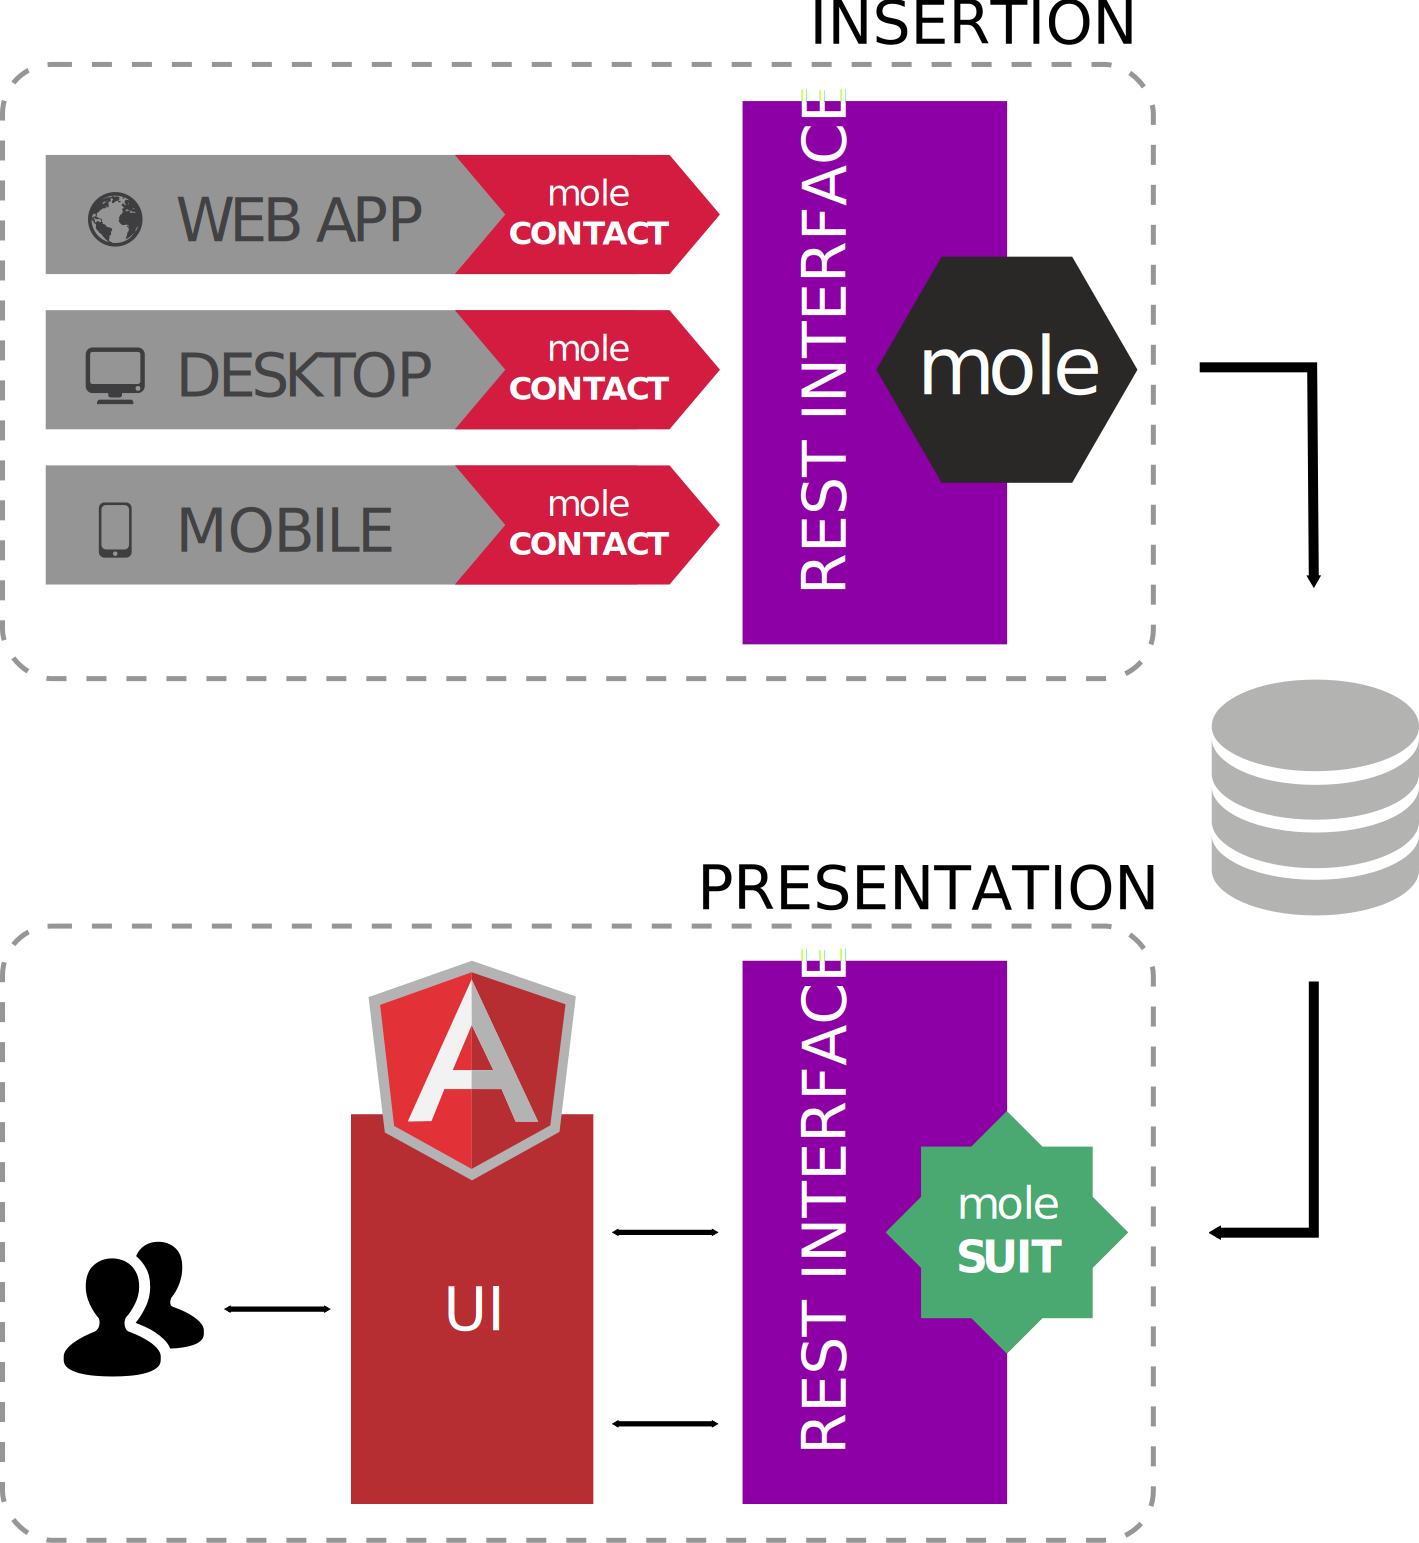
\includegraphics[width=1.0\linewidth]{./img/rest}
\caption[L'architettura di Mole.io]{L'architettura di Mole.io}
\label{fig:rest}
\end{figure}

In tabella \ref{tab:endpoint} sono riportati i principali endpoint delle interfacce REST esposte da ciascun componente in Mole.io. Per ciascun endpoint sono state riportate la tipologia di comando utilizzata per interagire con l'URI (\verb|GET| o \verb|POST|) e una descrizione delle funzionalit� offerte da esso.

\begin{table}[H]
\begin{center}
\begin{tabular}{|l|l|l|p{3.5cm}|}
\hline 
& \textbf{Tipo} & \textbf{Endpoint} & \textbf{Descrizione} \\
\hline
\multirow{3}{*}{\rotatebox[origin=c]{90}{\textbf{mole}}} & \verb|POST| & \verb|/whispers| & permette ai mole-contact di inviare whisper a mole \\
\hline
\multirow{14}{*}{\rotatebox[origin=c]{90}{\textbf{mole-suit}}} & \verb|GET| & \verb|/sources| & restituisce l'elenco delle source \\
\cline{2-4}
& \verb|POST| & \verb|/sources| & permette di inserire una nuova source \\
\cline{2-4}
& \verb|GET| & \verb|/sources/sID| & restituisce i dati della source con id \verb|sID| \\
\cline{2-4}
& \verb|GET| & \verb|/sources/sID/whispers| & restituisce l'elenco degli whisper ricevuti dalla source con id \verb|sID| \\
\cline{2-4}
& \verb|GET| & \verb|/sources/sID/whispers/wID| & restituisce l'elenco al whisper con id \verb|wID| ricevuto dalla source con id \verb|sID| \\
\hline
\end{tabular}
\caption{I principali endpoint REST forniti da Mole.io}\label{tab:endpoint}
\end{center}
\end{table}

Implementare una interfaccia REST con Node.js � piuttosto semplice, specialmente se si utilizza il modulo Express, descritto nella sezione \ref{Npm_e_moduli}. Express, infatti, mette a disposizione dello sviluppatore un sistema molto potente di \textit{route}, che permettono di identificare la risorsa desiderata a fronte di una richiesta in arrivo. Il codice seguente implementa un esempio di rotta con Express.\\

\begin{verbatim}
var express = require('express');
var app = express();
app.use(app.router);
app.get('/now', function(req, res) {
  res.json({ now: new Date().toString() });
});
\end{verbatim}

L'applicazione Node.js carica il modulo Express e genera una applicazione utilizzando tale modulo. Successivamente viene registrata una rotta che corrisponde all'URI \verb|/now|. All'arrivo di una richiesta di tipo \verb|GET| verso la risorsa \verb|/now|, Express esegue la callback associata e restituisce un documento JSON simile a quello seguente.
\begin{verbatim}
{ "now": "Sun Mar 09 2014 20:48:35 GMT+0100 (CET)" }
\end{verbatim}

Il \textit{router} Express, come molti altri plugin di questo sistema, rappresenta un \textit{middleware}. Il comando \verb|app.use(app.router);|, infatti, indica ad Express di utilizzare il middleware \verb|router| per filtrare le richieste in arrivo.

Un middleware � un modulo software che filtra ogni richiesta in arrivo dai client. I middleware cooperano tra loro e vengono attivati in successione. Il flusso di lavoro di un middleware � riassumibile in tre fasi principali:

\begin{enumerate}
\item ottenere la richiesta;
\item validare la richiesta ed eseguire funzionalit� specifiche associate al middleware stesso;
\item passare la richiesta al prossimo middleware;
\end{enumerate}

Seguendo il medesimo schema di funzionamento, i middleware, elaborano le risposte provenienti dall'applicazione e restituite al client. La figura \ref{fig:middleware} illustra il funzionamento di questo sistema.

\begin{figure}[H]
\centering
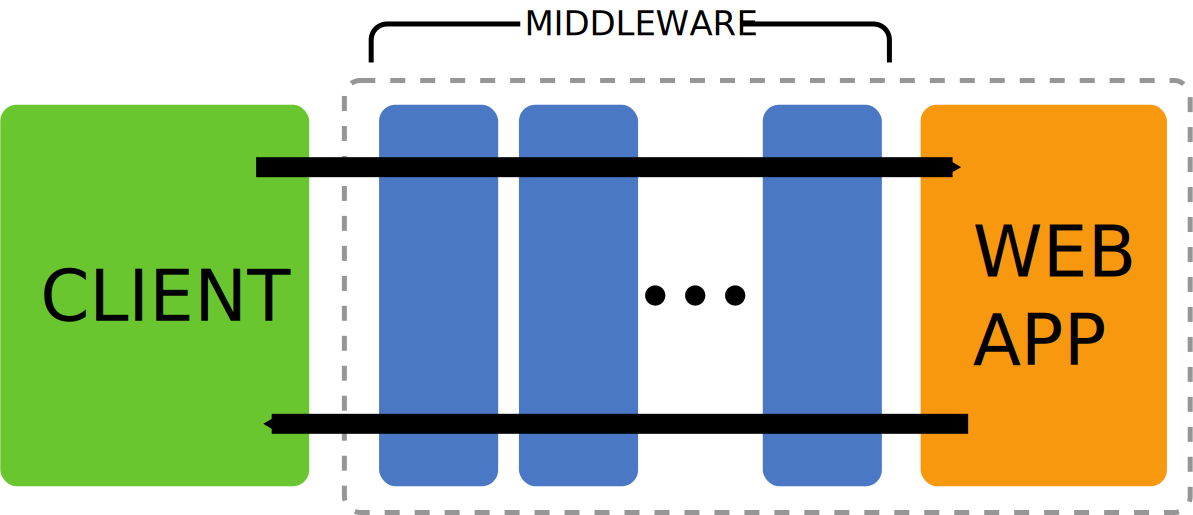
\includegraphics[width=1.0\linewidth]{./img/middleware}
\caption[Schema di funzionamento dei middleware]{Schema di funzionamento dei middleware}
\label{fig:middleware}
\end{figure}

%Nell'architettura di Mole.io si possono innanzitutto individuare quattro macro-componenti principali: \textit{mole-contact}, \textit{mole}, \textit{mole-suit} e il frontend o \textit{user-interface} (UI). Nella sezione \ref{Moleio} sono stati introdotti alcuni di questi attori, definendo la genesi dei rispettivi nomi. I componenti mole e mole-suit, sono server web realizzati in Node.js e utilizzano interfacce di tipo REST per comunicare con i client, rispettivamente i mole-contact e la UI.
%La tabella \ref{tab:endpoint}, introduce un nuovo concetto: le \textit{source}. Una source �, come suggerisce il nome, una sorgente di informazioni per Mole.io o, per meglio identificare il ruolo della source, una sorgente di whisper.
%Secondo la nomenclatura adottata in Mole.io, una source � infatti una applicazione contenente un mole-contact. Mole.io � in grado di interagire con svariate tipologie di applicazioni: web, desktop oppure mobile. L'unico requisito necessario � la possibilit� di utilizzare comunicazioni di rete per permettere al mole-contact di contattare il server mole. 
%Questo \textit{layer} dell'applicazione si occupa dell'inserimento dei dati nel sistema e si avvale di diversi moduli per fare in modo che gli whisper vengano salvati, aggregati e organizzati nel database.
%Nello schema \ref{} � riportata l'architettura del layer di insertion, essa � composta da diversi moduli:
%mole-contacts
%la porzione di sistema che si occupa dell'inserimento dei dati provenienti dall'esterno, � composta a sua volta dai \textit{mole-contacts}, da \textit{mole} e dai \textit{denormalizers}.

	\clearpage
		\subsection{CQRS ed Estensibilit�}\label{CQRS_ed_estensibilita}
		%TODO
% cosa è CQRS
% come Mole.io implementa il pattern

% preblema del read/write lock di mongo (qui o sulla scalabilità?)

		\clearpage
		\subsection{Mole}\label{mole}
		\clearpage
			\subsubsection{I Denormalizzatori}\label{I_denormalizzatori}
			\clearpage
		\subsection{Mole Suit}\label{mole-suit}
		\clearpage
			\subsubsection{I Plugin e gli Widget}\label{I_plugin_e_gli_widget}
			\clearpage
	\section{Autenticazione degli Utenti}\label{Autenticazione_degli_utenti}
	\clearpage
	\section{Scalabilit� e Affidabilit�}\label{Scalabilita_e_affidabilita}
	\clearpage
	\section{Problematiche di Sviluppo}\label{Problematiche_di_sviluppo}
	\clearpage

\chapter{Configurazioni e Benchmark}\label{Configurazioni_e_benchmark}
problemi con i benchmark
- dipendi dalla rete su cui sei
- nostro client fatto con node - perch� non l'abbiamo usato
- 2 parole sul tool che abbiamo usato
- come sono stati fatti i benchmark
- specifiche del sistema VM, ram, hdd, ...
- risultati ottenuti


non ha senso testare mole (server) per la parte rabbit (spiegare)
il vero collo di bottiglia � il db
abbiamo testato con configurazioni di db differenti

% parlare dei casini con le chiavi di shard



\clearpage

\chapter*{Conclusioni e Sviluppi Futuri\markboth{}{Conclusioni e Sviluppi Futuri}}\label{Conclusioni_e_sviluppi_futuri}
\addcontentsline{toc}{chapter}{Conclusioni e sviluppi futuri}
testere il sistema "in piccolo" � difficile, provare test sul sistema deployato

%TODO
% workflow con webhooks
% notifiche push (si potrebbe usare un denormalizer?)
% app mobile per riceverle
% https
% marcatura degli errori come "gestito" e conseguente archiviazione
% integrazione con sistemi di tracking (?)
% aggiungere pi� mole-contacts
% aggiungere un sistema di query
% mole-contacts -> caching degli errori in locale quando non c'� rete (buffering)

% migliorare la gestione dgli widget e plugin per l'aggiunta a caldo

% possibili nuovi denormalizzatori

% bench e vm sulla stessa macchina
% vm con cpu pin
% ramp up

\clearpage

%\end{comment}

\bibliography{Bibliografia}
\bibliographystyle{unsrt}
\addcontentsline{toc}{chapter}{Bibliografia}

\end{document}

%
%il problema
%- problema del logging:
%  - tante applicazioni
%  - diversi clienti
%  - report errori
%
%stato dell'arte: i software di logging centralizzato
%- aircoso
%- fluentd + elastic search + kibana
%perch\'{e} lo stato dell'arte non ci piace
%- non permettono di avere "modelli/template di messaggi" flessibili
%- contesti differenti
%
%il nostro logger 
%- perch\'{e} abbiamo scelto nodejs
%- cos'� nodejs (storia, peculiarit�, async, pesca da presentazione lucio)
%- come funziona il logger (struttura e schema delle comunicazioni di rete)
%- problematiche incontrate durante l'implementazione
%- si auto-adatta al tipo di messaggio in arrivo
%- denormalizzatori
%- plugin/widget
%- il clAud
%- architettura del sistema
%- estensibilit�
%- come scrivere plugin e widget
%
%problematiche "accademiche"
%- sicurezza (oauth)
%- scalabilit� (+ server con load balancer? cloud? rabbit, disaccoppiamento dei servizi)
%- relayability (+ server ridondati) 
%
%
%
%Scaletta:
%
%Metodologie:
% - CQRS
% - TDD
% - user stories
%
%Tecnologie utilizzate:
%- NodeJS
%  - npm (gestione dipendenze)
%  - passport (oauth)
%  - mongoskin
%  - mongoose
%  - underscore
%  - express
%  - faker (fixtures)
%  - grunt (automation)
%  - mocha (testing)
%  - should (testing)
%  - supertest (testing)
%  - require-all (plugin)
%  - cors (e problemi correlati)
%
%- rabbitmq
%
%- angularjs
%  - leflet (mappe)
%  - directive
%  - controller
%  - views
%  - services
%  - filters
%  - karma (testing)
%  - d3 (grafici)
%  - jquery
%  - bootstrap (ui)
%  - bower (gestione dipendenze)
%
%- mongodb
%  - sharding
%  - replicaset
%
%- dokku
%  
%- git(?)





